% CO3135 - Đánh giá kết quả phân loại truyền thống và học sâu.
% Tương thích để chèn bằng \input{phan_loai_va_danh_gia} trong main.tex.
% Không cần lệnh riêng \plot, \metric hay môi trường criticalnote.
% Các package cần dùng được liệt kê trong HUONG_DAN_OVERLEAF.md.
% Phần đánh giá kết quả phân loại truyền thống và học sâu.
% Được thiết kế để chèn bằng \input vào báo cáo chung, không tự tạo mục lục hoặc phụ lục.
\section{Đánh giá hiệu năng phân loại trên đặc trưng truyền thống và đặc trưng học sâu}
\label{sec:classification-evaluation}
% Phan noi dung co the input vao bao cao chung.
% Khong chua bia, thong tin sinh vien hay cac ket qua final test chua co.

\subsection{Phạm vi và mục tiêu đánh giá}
\label{sec:scope}
Nghiên cứu đánh giá hiệu năng phân loại ảnh rác thải gia dụng thành 12 lớp với hai nhóm đặc trưng: (i) đặc trưng truyền thống gồm HOG, SIFT kết hợp Bag of Visual Words (BoVW) và HOG kết hợp histogram màu HSV; (ii) đặc trưng học sâu trích xuất từ ResNet50, EfficientNet-B0 và ViT-B/16 tiền huấn luyện trên ImageNet. Các mạng học sâu được giữ cố định trọng số và chỉ dùng để trích xuất đặc trưng, không được huấn luyện lại trên bộ dữ liệu rác thải. Cả hai hướng đều sử dụng các bộ phân loại học máy gồm Logistic Regression (LR), Support Vector Machine (SVM) và Random Forest (RF). Đơn vị so sánh là một cấu hình hoàn chỉnh gồm đặc trưng, các bước tiền xử lý và bộ phân loại.

Thực nghiệm tập trung trả lời bốn câu hỏi: các loại đặc trưng và bộ phân loại khác nhau cho hiệu năng như thế nào?; điều chỉnh siêu tham số ảnh hưởng ra sao đến kết quả?; các lớp nào thường bị nhầm lẫn?; và PCA tạo ra sự đánh đổi như thế nào giữa số chiều, hiệu năng phân loại và chi phí tính toán?. Các kết quả trong phần này phục vụ khảo sát và lựa chọn mô hình trên tập development, không phải kết quả trên tập kiểm tra cuối cùng.

\subsection{Thiết lập thực nghiệm và chỉ số đánh giá}
\label{sec:protocol}
\subsubsection{Dữ liệu và biểu diễn đặc trưng}
Bộ dữ liệu sau khi làm sạch và loại ảnh trùng gồm 15\,866 ảnh thuộc 12 lớp. Trong đó, tập development (dev) gồm 12\,692 ảnh, tương ứng khoảng 80\% dữ liệu (10\,153 ảnh train và 2\,539 ảnh validation ở lần chia ban đầu). Tập kiểm tra cuối cùng (final test) gồm 3\,174 ảnh còn lại, được giữ riêng và không dùng để lựa chọn mô hình.

\begin{table}[H]\centering
\caption{Các loại đặc trưng được sử dụng trong hai hướng phân loại.}
\label{tab:features}
\small\begin{tabularx}{\linewidth}{@{}lclX@{}}\toprule
Nhánh & Đặc trưng & Số chiều & Bản chất và lưu ý\\\midrule
Truyền thống & HOG & 8\,100 & Phân bố hướng gradient trên ảnh xám 128$\times$128; không trực tiếp sử dụng thông tin màu.\\
Truyền thống & SIFT-BoVW & 500 & Histogram của các từ thị giác (visual words) tạo từ đặc trưng dense SIFT trên ảnh 224$\times$224; từ điển được học bằng \texttt{MiniBatchKMeans}.\\
Truyền thống & HOG + màu & 8\,228 & Ghép HOG với histogram màu HSV 128 chiều sau khi chuẩn hóa L2 từng nhóm đặc trưng.\\
Học sâu & ResNet50 & 2\,048 & Vector đặc trưng do CNN tiền huấn luyện trên ImageNet tạo ra.\\
Học sâu & EfficientNet-B0 & 1\,280 & Vector đặc trưng do CNN tiền huấn luyện trên ImageNet tạo ra.\\
Học sâu & ViT-B/16 & 768 & Vector đặc trưng từ Vision Transformer tiền huấn luyện trên ImageNet.\\\bottomrule
\end{tabularx}
\end{table}

HOG và SIFT-BoVW sử dụng cách trích xuất và kích thước ảnh đầu vào khác nhau; ba mô hình trích xuất đặc trưng học sâu cũng khác về kiến trúc và số chiều. Do đó, phép so sánh giữa các cấu hình không cô lập riêng ảnh hưởng của một yếu tố nếu nhiều thành phần được thay đổi đồng thời.

\subsubsection{Quy trình huấn luyện và đánh giá}
Trên tập dev, các mô hình được đánh giá bằng kiểm định chéo phân tầng 5 fold (5-fold stratified cross-validation, CV) với \texttt{StratifiedKFold}, \texttt{shuffle=True} và \texttt{random\_state=42}. Ở mỗi lượt, bốn fold được dùng để huấn luyện và fold còn lại dùng để xác thực. Số ảnh xác thực lần lượt là 2\,539, 2\,539, 2\,538, 2\,538 và 2\,538. Đối chiếu mã MD5 của ảnh trên metadata hiện có xác nhận hai cách chia dữ liệu của hai hướng tạo ra cùng năm fold.

Các bước chuẩn hóa bằng \texttt{StandardScaler} và giảm chiều bằng PCA (nếu sử dụng) được đặt trong \texttt{Pipeline} để chỉ học tham số biến đổi từ phần huấn luyện. Hướng truyền thống lựa chọn cấu hình dựa trên kết quả của năm fold; hướng học sâu sử dụng một tập xác thực phân tầng bên trong mỗi fold huấn luyện để lựa chọn siêu tham số cho các cấu hình được khảo sát tiếp. Riêng từ điển BoVW đã được học trước CV; giới hạn của bước này được phân tích ở Mục~\ref{sec:threats}.

Dự đoán out-of-fold (OOF) là dự đoán của mỗi ảnh từ bộ phân loại không sử dụng ảnh đó trong phần huấn luyện của fold tương ứng. Các dự đoán OOF được gộp để phân tích kết quả theo từng lớp. Đối với SIFT-BoVW, việc học từ điển trước CV vẫn là một giới hạn của các dự đoán này.

\subsubsection{Các chỉ số đánh giá}
Do lớp \texttt{clothes} chiếm khoảng một phần ba số ảnh, Accuracy có thể cao ngay cả khi mô hình dự đoán kém ở các lớp ít mẫu. Vì vậy, Macro-F1 được chọn làm chỉ số đánh giá chính (primary evaluation metric), với trọng số bằng nhau cho $K=12$ lớp. Gọi $TP_c$, $FP_c$ và $FN_c$ lần lượt là số dự đoán dương tính đúng, dương tính sai và âm tính sai đối với lớp $c$. Precision và Recall của lớp $c$ được tính như sau:
\[
P_c=\frac{TP_c}{TP_c+FP_c},\qquad R_c=\frac{TP_c}{TP_c+FN_c}.
\]
\begin{equation}\label{eq:macro}
\mathrm{MacroF1}=\frac{1}{K}\sum_{c=1}^{K}\mathrm{F1}_c,\qquad
\mathrm{F1}_c=\frac{2P_cR_c}{P_c+R_c},\quad K=12.
\end{equation}

Các chỉ số có mẫu số bằng 0 được quy ước bằng 0. Accuracy là tỷ lệ dự đoán đúng trên tổng số ảnh; Macro-Precision và Macro-Recall là trung bình cộng Precision và Recall của 12 lớp. Các chỉ số theo từng lớp và ma trận nhầm lẫn được sử dụng để phân tích lỗi phân loại.

Kết quả CV được tổng hợp qua năm fold dưới dạng trung bình $\pm$ độ lệch chuẩn (SD). Gọi $m_i$ là giá trị chỉ số ở fold thứ $i$ và $\bar m=\frac{1}{5}\sum_{i=1}^{5}m_i$. Để giữ nhất quán với kết quả và biểu đồ đã lưu, hướng truyền thống sử dụng $\mathrm{SD}=\sqrt{\frac{1}{5}\sum_{i=1}^{5}(m_i-\bar m)^2}$ (\texttt{ddof=0}), còn hướng học sâu sử dụng $\mathrm{SD}=\sqrt{\frac{1}{4}\sum_{i=1}^{5}(m_i-\bar m)^2}$ (\texttt{ddof=1}). Do khác quy ước, không so sánh trực tiếp hai giá trị SD mà không quy đổi. SD chỉ mô tả mức biến động giữa các fold; các tập huấn luyện chồng lặp nên không thể xem năm fold là năm quan sát độc lập hoặc diễn giải SD như khoảng tin cậy. Macro-F1 trung bình qua năm fold cũng không nhất thiết bằng Macro-F1 tính trên toàn bộ dự đoán OOF gộp.

Đối với thí nghiệm PCA, các đại lượng bổ sung gồm số chiều, tỷ lệ phương sai được giữ lại, dung lượng lưu trữ mỗi vector và thời gian huấn luyện hoặc dự đoán trên đặc trưng đã trích xuất (nếu có số liệu). Các phép đo thời gian không đại diện cho toàn bộ quy trình từ ảnh đầu vào đến nhãn dự đoán.

\subsection{Đánh giá kết quả phân loại với đặc trưng truyền thống}
\label{sec:traditional}

\subsubsection{Kết quả ban đầu và dấu hiệu quá khớp}
\label{subsec:tradbase}
Để xác định mức tham chiếu, hai chiến lược của \texttt{DummyClassifier} được đánh giá trước khi huấn luyện Logistic Regression (\texttt{C=1}, \texttt{class\_weight=balanced}) trên HOG và SIFT-BoVW. Với \texttt{most\_frequent}, mô hình luôn dự đoán lớp phổ biến nhất; với \texttt{stratified}, nhãn được lấy ngẫu nhiên theo phân bố ước lượng từ tập huấn luyện của từng fold.

\begin{table}[H]\centering\caption{Kết quả đánh giá ban đầu của hướng truyền thống trên \textit{development} (5-fold CV).}\label{tab:tradbase}
\small\begin{tabular}{@{}llcc@{}}\toprule
Bộ phân loại & Đặc trưng & Macro-F1 ($\bar m\pm\mathrm{SD}$) & Accuracy\\\midrule
Dummy - most frequent & Không dùng & 0.0416 $\pm$ 0.0000 & 0.3331\\
Dummy - stratified & Không dùng & 0.0793 $\pm$ 0.0038 & 0.1561\\
Logistic Regression & SIFT-BoVW & 0.4600 $\pm$ 0.0089 & 0.5635\\
Logistic Regression & HOG & 0.3234 $\pm$ 0.0083 & 0.4656\\\bottomrule
\end{tabular}\end{table}

Bảng~\ref{tab:tradbase} cho thấy Dummy most-frequent đạt Accuracy $0.3331$ nhưng Macro-F1 chỉ $0.0416$, minh họa hạn chế của Accuracy khi dữ liệu mất cân bằng. Với LR, SIFT-BoVW đạt Macro-F1 cao hơn HOG khoảng 13.66 điểm phần trăm. Trên HOG, Macro-F1 huấn luyện đạt $1.0000$, trong khi Macro-F1 xác thực chỉ đạt $0.3234$, tạo khoảng cách 67.66 điểm phần trăm. Đây là dấu hiệu quá khớp (overfitting) và là cơ sở để khảo sát mức chính quy hóa (regularization).

\subsubsection{Ảnh hưởng của điều chỉnh siêu tham số trên SIFT-BoVW}
\label{subsec:sift}
\paragraph{Logistic Regression và tham số $C$}\mbox{}\par
LR đa lớp được huấn luyện trên histogram BoVW 500 chiều. Với regularization L2, $C$ nhỏ tương ứng mức phạt lớn hơn đối với hệ số mô hình. Thí nghiệm so sánh Macro-F1 huấn luyện và xác thực tại các giá trị:
\[C\in\{0.001,0.002,0.005,0.01,0.05,0.1,1,10\}.\]

\begin{figure}[H]
    \centering
    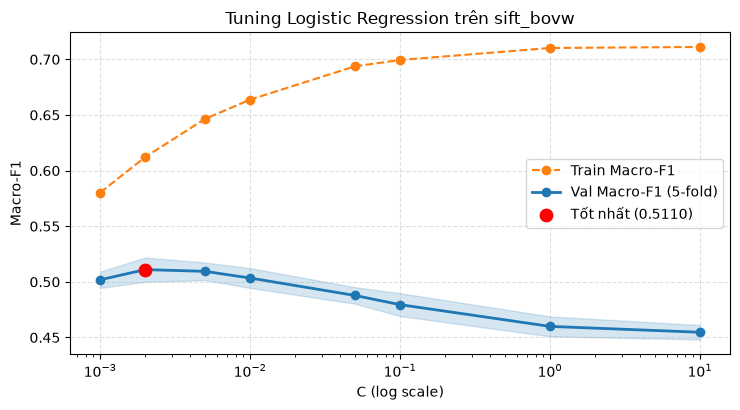
\includegraphics[width=0.89\linewidth]{figures/trad_cell07_out2.png}
    \caption{Macro-F1 trên \textit{train} và \textit{validation} của Logistic Regression theo giá trị $C$ trên SIFT-BoVW.}
    \label{fig:sift-lr}
\end{figure}

Từ Hình~\ref{fig:sift-lr}, khi giảm $C$ từ $10$ xuống $0.002$, Macro-F1 huấn luyện giảm từ $0.7111$ xuống $0.6122$ nhưng Macro-F1 xác thực tăng từ $0.4547$ lên $0.5110\pm0.0109$. Giảm tiếp xuống $C=0.001$ làm Macro-F1 xác thực giảm còn $0.5019$. Trong lưới khảo sát, $C=0.002$ cho kết quả xác thực cao nhất; kết quả này minh họa vai trò của regularization trong việc hạn chế quá khớp.

\paragraph{LinearSVC và SVM RBF}\mbox{}\par
Cùng trên SIFT-BoVW, LinearSVC đạt $0.5028\pm0.0132$ tại $C=0.005$. Với SVM sử dụng hàm nhân RBF, Macro-F1 đạt $0.5718\pm0.0041$ ở $C=10$, $\gamma=\texttt{scale}$. Đường biểu diễn dưới đây cho phép theo dõi kết quả huấn luyện và xác thực khi thay đổi $C$.

\begin{figure}[H]
    \centering
    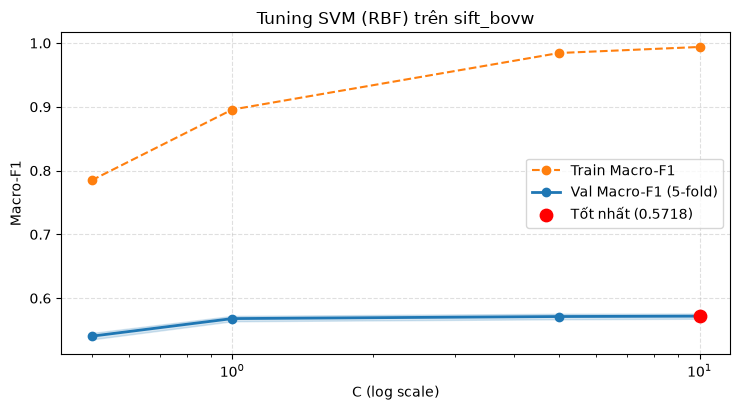
\includegraphics[width=0.89\linewidth]{figures/trad_cell08_out2.png}
    \caption{Macro-F1 của SVM RBF theo $C$ trên SIFT-BoVW}
    \label{fig:sift-rbf}
\end{figure}

Hình~\ref{fig:sift-rbf} cho thấy khi tăng $C$ từ $0.5$ lên $10$, Macro-F1 huấn luyện tăng từ $0.7847$ lên $0.9939$, trong khi Macro-F1 xác thực tăng từ $0.5404$ lên $0.5718$. Từ $C=1$ đến $C=10$, mức cải thiện trên tập xác thực chỉ còn 0.38 điểm phần trăm, đồng thời khoảng cách giữa huấn luyện và xác thực tiếp tục tăng. Trong lưới $C\in\{0.5,1,5,10\}$, $C=10$ đạt Macro-F1 xác thực trung bình cao nhất; chưa có kết quả cho các giá trị lớn hơn.

\paragraph{Random Forest và đối chiếu các bộ phân loại}\mbox{}\par
Với Random Forest, nghiên cứu khảo sát \texttt{n\_estimators}, \texttt{max\_depth}, \texttt{max\_features} và \texttt{class\_weight}. Cấu hình \texttt{n\_estimators=200}, \texttt{max\_depth=15} đạt Macro-F1 $0.4899\pm0.0142$. Khi không giới hạn độ sâu cây, Macro-F1 huấn luyện gần $1.0000$, trong khi Macro-F1 xác thực chỉ khoảng $0.4808$. Đây là dấu hiệu quá khớp khi tăng khả năng khớp dữ liệu của từng cây quyết định trong cấu hình đã thử.

\begin{table}[H]\centering\caption{Cấu hình đạt Macro-F1 cao nhất của từng bộ phân loại trên SIFT-BoVW.}\label{tab:siftbest}
\small\begin{tabularx}{\linewidth}{@{}lXcc@{}}\toprule
Bộ phân loại & Siêu tham số được chọn & Macro-F1 & Accuracy\\\midrule
LR & $C=0.002$, balanced & $0.5110\pm0.0109$ & 0.6079\\
LinearSVC & $C=0.005$, balanced & $0.5028\pm0.0132$ & 0.6181\\
SVM RBF & $C=10$, $\gamma=\texttt{scale}$, balanced & \textbf{$0.5718\pm0.0041$} & 0.6791\\
RF & 200 cây, \texttt{max\_depth=15}, \texttt{max\_features=sqrt}, \texttt{balanced\_subsample} & $0.4899\pm0.0142$ & 0.5947\\\bottomrule
\end{tabularx}\end{table}

Trên cùng đặc trưng SIFT-BoVW, SVM RBF đạt Macro-F1 cao hơn LR 6.08 điểm phần trăm và cao hơn LinearSVC 6.90 điểm phần trăm trong phạm vi các cấu hình đã khảo sát.

\subsubsection{Điều chỉnh siêu tham số trên đặc trưng HOG}
\label{subsec:hog}
Nghiên cứu khảo sát Logistic Regression, SVM tuyến tính và Random Forest; SVM tuyến tính trên HOG được triển khai bằng \texttt{SGDClassifier} với \texttt{loss=hinge} và \texttt{penalty=l2}, thay cho \texttt{LinearSVC} để giảm chi phí tính toán. Vì thuật toán tối ưu khác nhau, không thể quy mọi chênh lệch giữa HOG và SIFT-BoVW cho riêng loại đặc trưng.

\begin{figure}[H]\centering
\begin{subfigure}[t]{0.485\linewidth}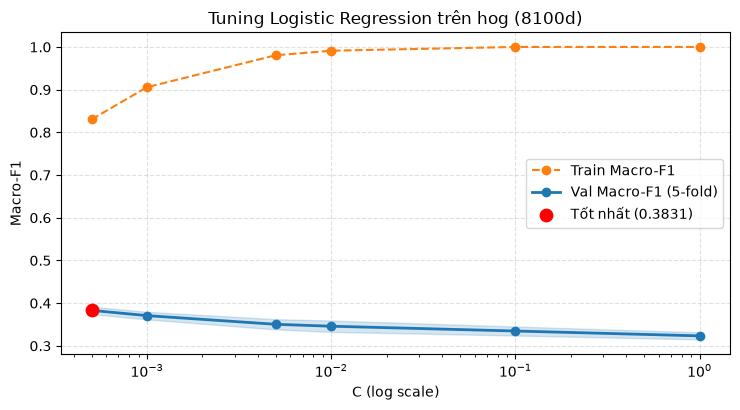
\includegraphics[width=\linewidth]{figures/trad_cell12_out2.png}\caption{LR trên HOG.}\end{subfigure}\hfill
\begin{subfigure}[t]{0.485\linewidth}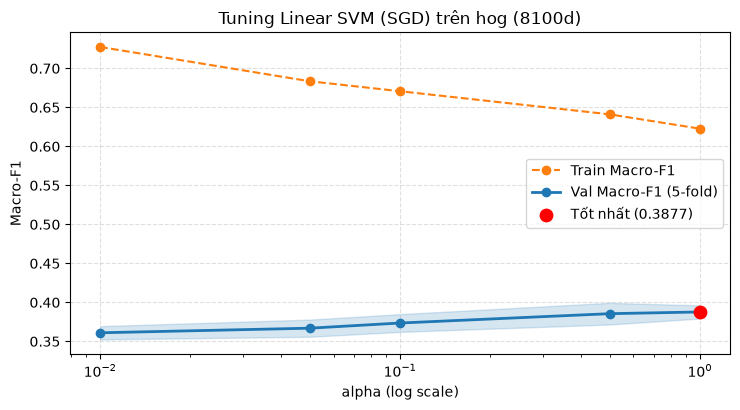
\includegraphics[width=\linewidth]{figures/trad_cell13_out2.png}\caption{SVM tuyến tính (SGD).}\end{subfigure}
\caption{Macro-F1 trên \textit{train} và \textit{validation} khi thay đổi mức chính quy hóa trên HOG.}\label{fig:hog-tuning}
\end{figure}

Hình~\ref{fig:hog-tuning} minh họa ảnh hưởng của regularization đối với LR và SVM tuyến tính. Giảm $C$ của LR từ $0.0005$ xuống $0.0001$ làm Macro-F1 xác thực tăng từ $0.3831$ lên $0.3953\pm0.0094$. So với LR ban đầu ($C=1$), khoảng cách Macro-F1 giữa huấn luyện và xác thực giảm từ 67.66 xuống 22.19 điểm phần trăm. Với SGDClassifier, $\alpha$ lớn hơn tương ứng mức chính quy hóa mạnh hơn; $\alpha=1$ đạt $0.3877\pm0.0084$, cao nhất trong các giá trị đã thử. Với RF, giảm \texttt{max\_depth} từ 15 xuống 10 giới hạn độ phức tạp của cây và làm Macro-F1 tăng từ $0.3484$ lên $0.3768\pm0.0102$.

\begin{table}[H]\centering\caption{Kết quả sau khi mở rộng lưới siêu tham số trên HOG}\label{tab:hogbest}
\small\begin{tabularx}{\linewidth}{@{}llXc@{}}\toprule
Bộ phân loại & Cấu hình tốt nhất ban đầu & Sau khi mở rộng & Macro-F1 sau khảo sát\\\midrule
LR & $C=0.0005$: 0.3831 & $C=0.0001$ & $0.3953\pm0.0094$\\
SVM (SGD) & $\alpha=1$: 0.3877 & Không thay đổi & $0.3877\pm0.0084$\\
RF & Độ sâu 15: 0.3484 & Độ sâu 10 & $0.3768\pm0.0102$\\\bottomrule
\end{tabularx}\end{table}

Các kết quả ở Bảng~\ref{tab:hogbest} cho thấy ba cấu hình HOG không PCA đạt Macro-F1 gần nhau và thấp hơn cấu hình SIFT-BoVW tốt nhất trong khảo sát. Việc mở rộng lưới giúp khảo sát thêm các giá trị khi cấu hình đạt kết quả cao nhất nằm ở biên lưới ban đầu. Các thí nghiệm PCA ở mục sau khảo sát thêm HOG kết hợp SVM RBF; kết quả của tổ hợp này không được xem là tác động của PCA riêng lẻ.

\subsubsection{So sánh sáu cấu hình và phân tích nhầm lẫn}
\label{subsec:traderror}
Để đối chiếu các kết quả sau điều chỉnh siêu tham số, Bảng~\ref{tab:trad-six} tập hợp sáu cấu hình tương ứng với ba nhóm bộ phân loại và hai loại đặc trưng truyền thống, khi chưa áp dụng PCA.

\begin{table}[H]\centering\caption{Kết quả tốt nhất theo từng cặp bộ phân loại và đặc trưng truyền thống}\label{tab:trad-six}
\small\begin{tabular}{@{}llccc@{}}\toprule
Đặc trưng & Bộ phân loại & Macro-F1 ($\bar m\pm\mathrm{SD}$) & Accuracy & Huấn luyện (s/fold)\\\midrule
SIFT-BoVW & LR & $0.5110\pm0.0109$ & 0.6079 & 0.99\\
SIFT-BoVW & SVM RBF & \textbf{$0.5718\pm0.0041$} & 0.6791 & 208.33\\
SIFT-BoVW & RF & $0.4899\pm0.0142$ & 0.5947 & 0.84\\
HOG & LR & $0.3953\pm0.0094$ & 0.5176 & 92.32\\
HOG & SVM (SGD) & $0.3877\pm0.0084$ & 0.5351 & 14.58\\
HOG & RF & $0.3768\pm0.0102$ & 0.5190 & 65.41\\\bottomrule
\end{tabular}\end{table}

Ở cả ba họ bộ phân loại, các cấu hình SIFT-BoVW đạt Macro-F1 cao hơn cấu hình HOG tương ứng. Trên HOG chưa giảm chiều, Macro-F1 của ba họ bộ phân loại chỉ dao động từ $0.3768$ đến $0.3953$. SVM RBF trên SIFT-BoVW có Macro-F1 cao nhất nhưng cũng có thời gian huấn luyện trung bình lớn hơn các cấu hình còn lại trong Bảng~\ref{tab:trad-six}. Do các cấu hình sử dụng số chiều và cách triển khai SVM khác nhau, sự khác biệt về thời gian không thể quy riêng cho loại đặc trưng.

\begin{figure}[H]\centering
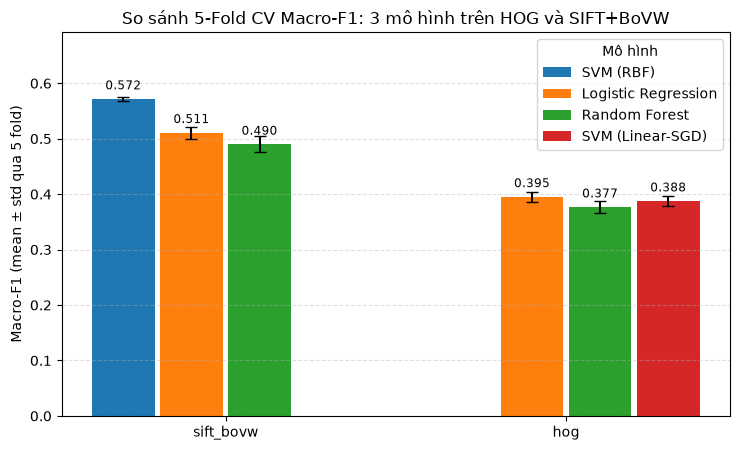
\includegraphics[width=0.92\linewidth]{figures/trad_cell19_out3.png}
\caption{So sánh Macro-F1 giữa các bộ phân loại trên HOG và SIFT-BoVW.}\label{fig:trad-six}
\end{figure}

Để xác định các lớp có hiệu năng thấp, nghiên cứu phân tích ma trận nhầm lẫn và F1 theo lớp từ dự đoán OOF của cấu hình có Macro-F1 cao nhất trên mỗi loại đặc trưng chưa giảm chiều.
\begin{figure}[H]
\centering
\begin{subfigure}[t]{0.52\linewidth}
\centering
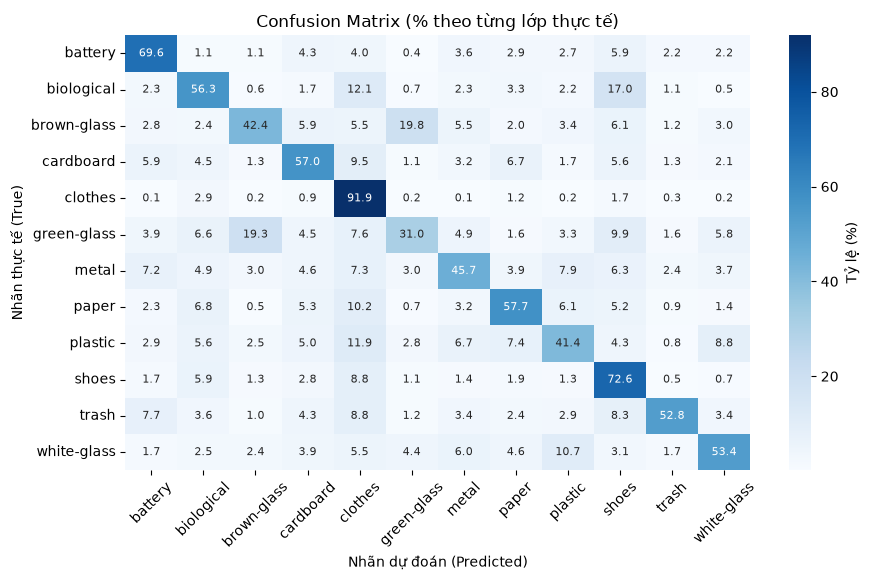
\includegraphics[width=\linewidth]{figures/trad_cell20_out1_panel1.png}
\caption{Ma trận nhầm lẫn OOF.}
\end{subfigure}\hfill
\begin{subfigure}[t]{0.45\linewidth}
\centering
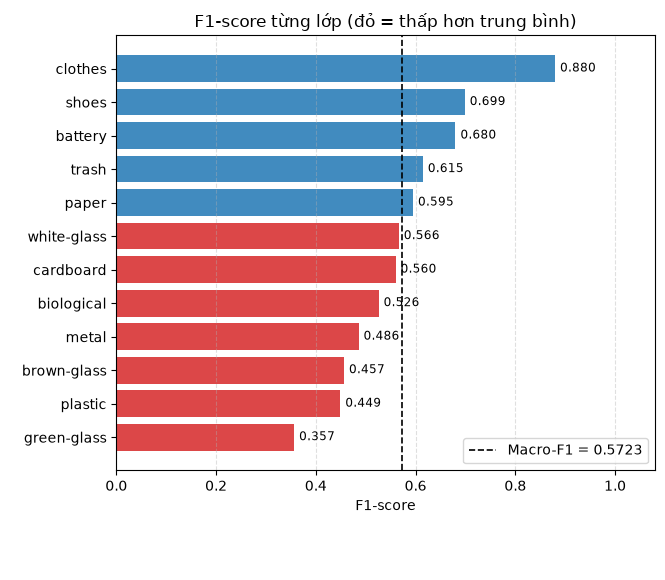
\includegraphics[width=\linewidth]{figures/trad_cell20_out1_panel2.png}
\caption{F1 theo từng lớp.}
\end{subfigure}
\caption{Phân tích lỗi của SIFT-BoVW + SVM RBF.}
\label{fig:trad-cm-sift}
\end{figure}

Ở cấu hình này, lớp \texttt{green-glass} có F1 khoảng $0.357$ và Recall $31.0\%$: $19.3\%$ ảnh thuộc lớp này bị dự đoán là \texttt{brown-glass}. Theo chiều ngược lại, khoảng $19.8\%$ ảnh \texttt{brown-glass} bị dự đoán thành \texttt{green-glass}. Với \texttt{white-glass}, tỷ lệ bị dự đoán thành \texttt{plastic} khoảng $10.7\%$. Ma trận nhầm lẫn cho biết hướng nhầm lẫn; biểu đồ F1 giúp nhận ra những lớp có kết quả thấp hơn trung bình.

Đối với HOG + Logistic Regression, ma trận OOF được trình bày riêng tại Hình~\ref{fig:trad-cm-hog} để kiểm tra xem các lớp khó có trùng với SIFT-BoVW hay không.

\begin{figure}[H]\centering
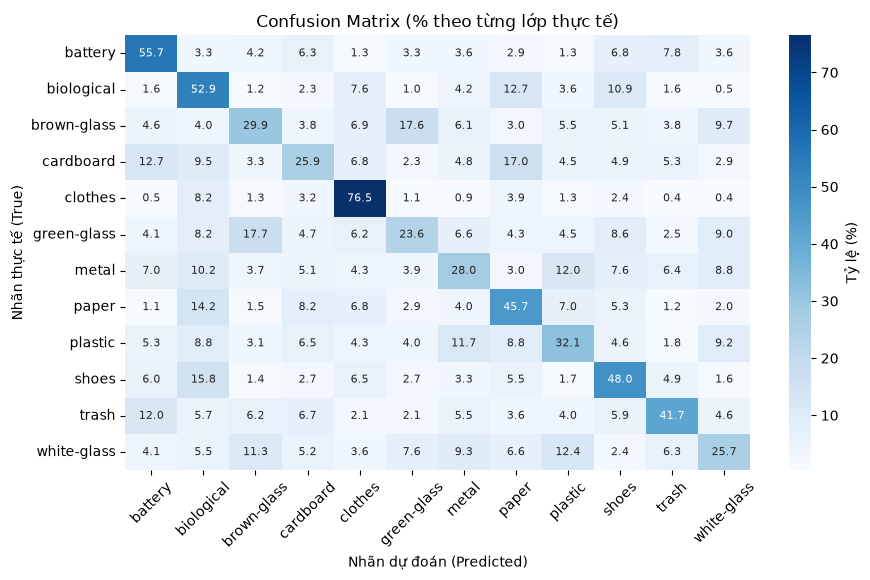
\includegraphics[width=0.80\linewidth]{figures/trad_cell20_out3_panel1.png}
\caption{Ma trận nhầm lẫn OOF của HOG + Logistic Regression sau điều chỉnh siêu tham số}\label{fig:trad-cm-hog}
\end{figure}

Cả hai cấu hình đều ghi nhận nhầm lẫn giữa các lớp thủy tinh và nhựa. Do bộ phân loại cũng khác nhau, chưa thể quy sự khác biệt trong ma trận nhầm lẫn riêng cho HOG hoặc SIFT-BoVW.

\subsubsection{Đánh giá ảnh hưởng của thông tin màu}
\label{subsec:color}
HOG và SIFT-BoVW trong thí nghiệm ban đầu được trích xuất từ ảnh xám. Để khảo sát việc bổ sung màu sắc, nghiên cứu giữ LR với $C=0.0001$ và so sánh HOG với HOG ghép histogram màu HSV 128 chiều. Hai nhóm đặc trưng được chuẩn hóa L2 riêng trước khi ghép.

Macro-F1 tăng từ $0.3953\pm0.0094$ lên $0.5040\pm0.0073$ (10.87 điểm phần trăm), còn Accuracy tăng từ $0.5176$ lên $0.5988$. Kết quả cho thấy cấu hình bổ sung thông tin màu có hiệu năng cao hơn. Tuy nhiên, phép ghép cũng thay đổi cách biểu diễn vector; chưa có kết quả theo từng lớp của HOG kết hợp màu để xác định mức cải thiện riêng đối với các lớp thủy tinh.

\subsubsection{Đánh giá ảnh hưởng của PCA}
\label{subsec:tradpca}
\paragraph{PCA trên HOG (8\,100 chiều)}\mbox{}\par
PCA được thực hiện sau \texttt{StandardScaler} trong phần huấn luyện của từng fold. Các cấu hình LR và SVM tuyến tính được đối chiếu với phiên bản không PCA. Riêng RF không PCA sử dụng đặc trưng chưa chuẩn hóa, trong khi RF có PCA sử dụng đặc trưng đã chuẩn hóa; do đó, phép so sánh RF đánh giá cả quy trình chuẩn hóa và giảm chiều, không cô lập riêng ảnh hưởng của PCA.

\begin{figure}[H]\centering
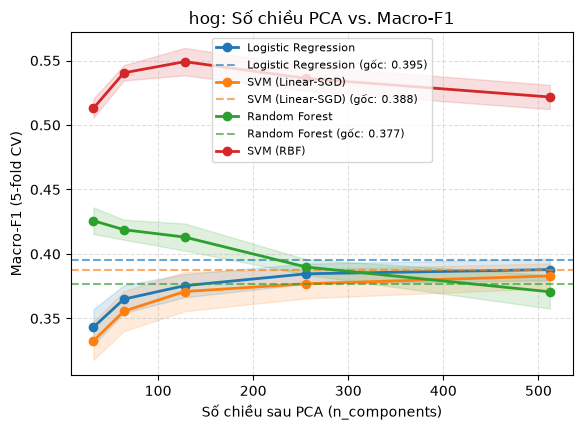
\includegraphics[width=0.8\linewidth]{figures/trad_cell24_out3_panel1.png}
\caption{Macro-F1 theo số thành phần PCA trên HOG, đối chiếu các bộ phân loại}\label{fig:hog-pca-perf}
\end{figure}

Với Logistic Regression, PCA 512 đạt $0.3879\pm0.0083$, thấp hơn cấu hình không PCA ($0.3953\pm0.0094$). SVM tuyến tính (SGD) với PCA 512 đạt $0.3830\pm0.0096$, gần với $0.3877\pm0.0084$ ở bản gốc. Random Forest kết hợp chuẩn hóa và PCA 32 đạt $0.4258\pm0.0103$, cao hơn mức $0.3768\pm0.0102$ khi không PCA; nhưng PCA 512 chỉ đạt $0.3707\pm0.0130$. Như vậy, ảnh hưởng của quy trình giảm chiều khác nhau giữa các bộ phân loại.

Một khảo sát bổ sung kết hợp HOG + PCA 128 với SVM RBF. Ở $C=5$, Macro-F1 đạt $0.5491\pm0.0106$; tăng $C$ lên $10$ cho $0.5499\pm0.0096$. 
\begin{figure}[H]\centering
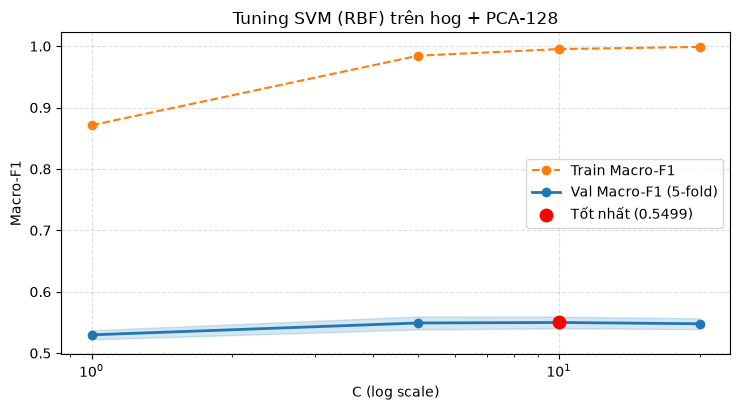
\includegraphics[width=0.9\linewidth]{figures/trad_cell28_out2.png}
\caption{Khảo sát bổ sung tham số $C$ của HOG + PCA 128 + SVM RBF.}\label{fig:hog-rbf-pca}
\end{figure}
Điểm số cao hơn HOG + Logistic Regression không chứng minh PCA tự nó làm tăng hiệu năng, vì tổ hợp này đồng thời sử dụng SVM RBF thay cho bộ phân loại tuyến tính. PCA giữ các hướng biến thiên lớn của dữ liệu, không trực tiếp lựa chọn các hướng phân biệt tốt nhất giữa 12 lớp.
\paragraph{PCA trên SIFT-BoVW (500 chiều)}\mbox{}\par
Với biểu diễn SIFT-BoVW, Hình~\ref{fig:sift-pca} cho thấy tác động của số thành phần PCA đối với Logistic Regression, SVM RBF và Random Forest.

\begin{figure}[H]\centering
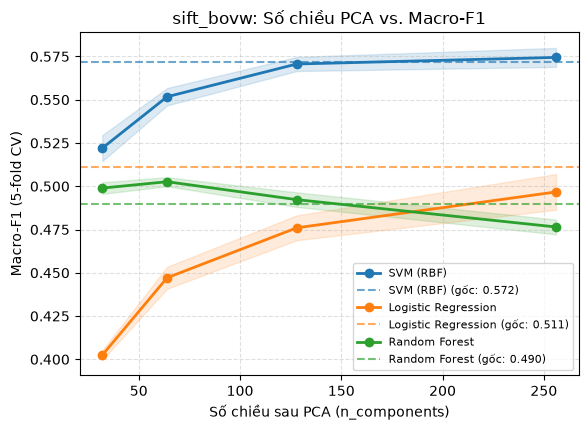
\includegraphics[width=0.8\linewidth]{figures/trad_cell25_out3_panel1.png}
\caption{Macro-F1 theo số thành phần PCA trên SIFT-BoVW của LR, SVM RBF và RF.}\label{fig:sift-pca}
\end{figure}

Khi giảm xuống PCA 256, Logistic Regression đạt $0.4967\pm0.0103$ so với $0.5110$ không PCA; giảm tiếp xuống PCA 32 còn $0.4025\pm0.0028$. Với SVM RBF, PCA 256 đạt $0.5744\pm0.0055$, gần với $0.5718\pm0.0041$ không PCA; PCA 128 đạt $0.5706\pm0.0041$. Random Forest kết hợp chuẩn hóa và PCA 64 đạt $0.5026\pm0.0026$, so với $0.4899\pm0.0142$ ở biểu diễn gốc.

\begin{table}[H]\centering\caption{Đối chiếu số chiều, Macro-F1 trung bình và thời gian huấn luyện của một số cấu hình truyền thống.}\label{tab:trad-pca-summary}
\small\begin{tabularx}{\linewidth}{@{}lXrcc@{}}\toprule
Đặc trưng & Bộ phân loại và PCA & Số chiều & Macro-F1 & Fit (s/fold)\\\midrule
HOG & LR, không PCA & 8\,100 & 0.3953 & 92.32\\
HOG & LR, PCA 512 & 512 & 0.3879 & 6.23\\
HOG & RF, không PCA & 8\,100 & 0.3768 & 65.41\\
HOG & RF, PCA 32 & 32 & 0.4258 & 15.58\\
HOG & SVM RBF, PCA 128 ($C=10$) & 128 & 0.5499 & 29.88\\\midrule
SIFT-BoVW & LR, không PCA & 500 & 0.5110 & 0.99\\
SIFT-BoVW & LR, PCA 256 & 256 & 0.4967 & 5.40\\
SIFT-BoVW & RF, không PCA & 500 & 0.4899 & 0.84\\
SIFT-BoVW & RF, PCA 64 & 64 & 0.5026 & 1.61\\
SIFT-BoVW & SVM RBF, không PCA & 500 & 0.5718 & 208.33\\
SIFT-BoVW & SVM RBF, PCA 256 & 256 & \textbf{0.5744} & 175.51\\
SIFT-BoVW & SVM RBF, PCA 128 & 128 & 0.5706 & 72.49\\\bottomrule
\end{tabularx}
\end{table}

Bảng~\ref{tab:trad-pca-summary} cho thấy HOG kết hợp LR giảm từ 8\,100 xuống 512 chiều (93.68\%) với mức giảm Macro-F1 0.74 điểm phần trăm. Trên SIFT-BoVW kết hợp SVM RBF, PCA 256 đạt Macro-F1 cao nhất trong phạm vi khảo sát, nhưng chênh lệch so với cấu hình không PCA chỉ khoảng 0.26 điểm phần trăm. PCA 128 giảm 74.4\% số chiều và chỉ giảm Macro-F1 khoảng 0.12 điểm phần trăm so với cấu hình 500 chiều, là một phương án đáng cân nhắc khi cần giảm dung lượng đặc trưng. Thời gian fit ghi nhận cũng thấp hơn, nhưng các cấu hình được đo ở những lượt chạy và mức song song có thể khác nhau. Các số liệu này chỉ mô tả thời gian huấn luyện pipeline trên đặc trưng đã trích xuất, không phải thời gian xử lý ảnh đầu vào.

\subsection{Đánh giá kết quả phân loại với đặc trưng học sâu}
\label{sec:deep}
\subsubsection{Kết quả ban đầu của chín tổ hợp bộ phân loại và đặc trưng học sâu}
\label{subsec:deepbase}
Ba loại vector đặc trưng học sâu được đưa vào LR, LinearSVC và RF. LR sử dụng $C=1$ và solver \texttt{lbfgs}; LinearSVC sử dụng $C=0.001$, \texttt{dual=True}, \texttt{max\_iter=5000}; RF sử dụng 100 cây, \texttt{max\_depth=None}, \texttt{max\_features=sqrt} và \texttt{min\_samples\_leaf=1}. LR và LinearSVC có bước \texttt{StandardScaler}, còn RF nhận vector chưa chuẩn hóa. Cả ba bộ phân loại không sử dụng trọng số lớp (\texttt{class\_weight=None}). Cả chín cấu hình dùng cùng năm fold.

Dummy most-frequent đạt Macro-F1 $0.0416$ và Accuracy $0.3331$. Các cấu hình kết hợp LR với đặc trưng học sâu đều đạt Macro-F1 cao hơn nhiều so với baseline này, cho thấy các vector trích xuất từ mô hình tiền huấn luyện mang thông tin hữu ích cho phân loại 12 lớp rác.

\begin{table}[H]\centering\caption{Chín tổ hợp bộ phân loại - biểu diễn học sâu trước điều chỉnh siêu tham số, Macro-F1 trung bình $\pm$ SD.}\label{tab:deep9}
\small\begin{tabular}{@{}lccc@{}}\toprule
Đặc trưng & Logistic Regression & LinearSVC & Random Forest\\\midrule
ResNet50 & $0.9272\pm0.0035$ & \textbf{$0.9417\pm0.0033$} & $0.9089\pm0.0070$\\
EfficientNet-B0 & $0.9401\pm0.0024$ & $0.9385\pm0.0064$ & $0.8883\pm0.0044$\\
ViT-B/16 & $0.9411\pm0.0033$ & $0.9410\pm0.0060$ & $0.8919\pm0.0067$\\\bottomrule
\end{tabular}\end{table}

\begin{figure}[H]
    \centering
    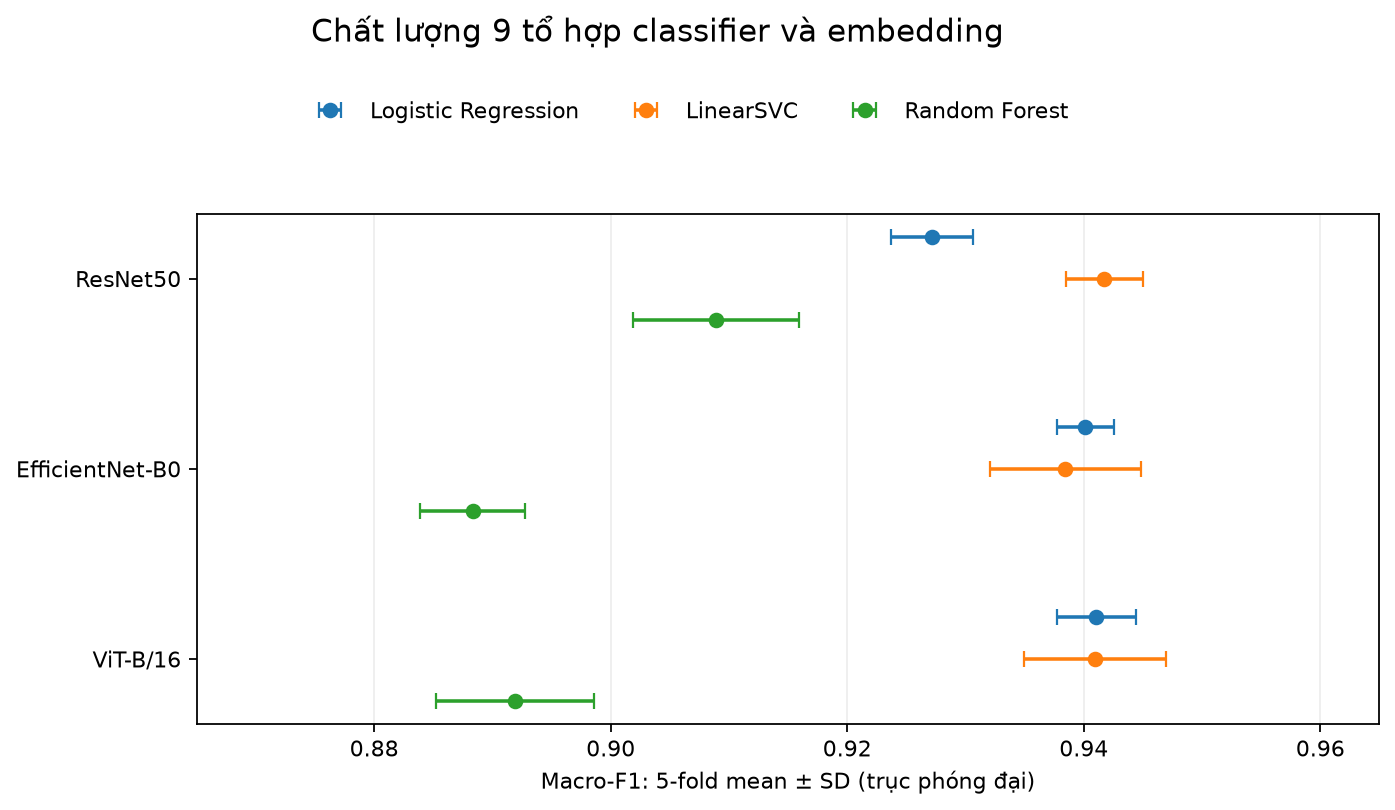
\includegraphics[width=0.97\linewidth]{figures/deep_cell11_out0.png}
    \caption{Macro-F1 của chín tổ hợp bộ phân loại và đặc trưng học sâu}
    \label{fig:deep-nine}
\end{figure}

LR và LinearSVC đạt Macro-F1 cao hơn RF trên cả ba loại đặc trưng học sâu trong các cấu hình ban đầu. ViT-B/16 đạt kết quả cao nhất với LR; ResNet50 đạt kết quả cao nhất với LinearSVC và RF. EfficientNet-B0 kết hợp LR cũng đạt kết quả gần với ViT-B/16. LinearSVC trên ResNet50 đạt Macro-F1 trung bình cao nhất, nhưng chỉ cao hơn LR trên ViT-B/16 khoảng 0.07 điểm phần trăm. Kết quả cho thấy thứ tự hiệu năng của các loại đặc trưng phụ thuộc vào bộ phân loại được sử dụng.

\subsubsection{Thay đổi hiệu năng sau điều chỉnh siêu tham số}
\label{subsec:deeptune}
Từ kết quả khảo sát ban đầu, ba cấu hình được chọn để điều chỉnh siêu tham số gồm LR + ViT-B/16, LinearSVC + ResNet50 và RF + ResNet50. Ở mỗi fold ngoài, \texttt{GridSearchCV} lựa chọn siêu tham số bằng một phép chia phân tầng bên trong: 20\% dữ liệu huấn luyện của fold ngoài được dành làm tập xác thực để so sánh theo Macro-F1. Sau bước lựa chọn, mô hình được huấn luyện lại trên toàn bộ phần huấn luyện của fold ngoài rồi mới dự đoán trên phần xác thực của fold đó. Lưới thử: $C\in\{0.1,1,10\}$ cho LR; $C\in\{0.0003,0.001,0.003\}$ cho LinearSVC; \texttt{min\_samples\_leaf}$\in\{1,2\}$ cho RF. Như vậy, việc chọn tham số dựa trên một phép chia xác thực bên trong cho mỗi fold ngoài, không phải kiểm định chéo nhiều fold ở vòng trong.

\begin{table}[H]\centering\caption{Macro-F1 trước và sau điều chỉnh siêu tham số của ba cấu hình học sâu, đánh giá trên năm fold ngoài.}\label{tab:deep-tune}
\small\begin{tabularx}{\linewidth}{@{}Xccc@{}}\toprule
Cấu hình & Trước tuning & Sau tuning ($\bar m\pm\mathrm{SD}$) & $\Delta$ (điểm \%)\\\midrule
LR + ViT-B/16 & 0.9411 & $0.9440\pm0.0037$ & $+0.29$\\
LinearSVC + ResNet50 & 0.9417 & \textbf{$0.9451\pm0.0030$} & $+0.34$\\
RF + ResNet50 & 0.9089 & $0.9061\pm0.0050$ & $-0.28$\\\bottomrule
\end{tabularx}\end{table}

\begin{figure}[H]
    \centering
    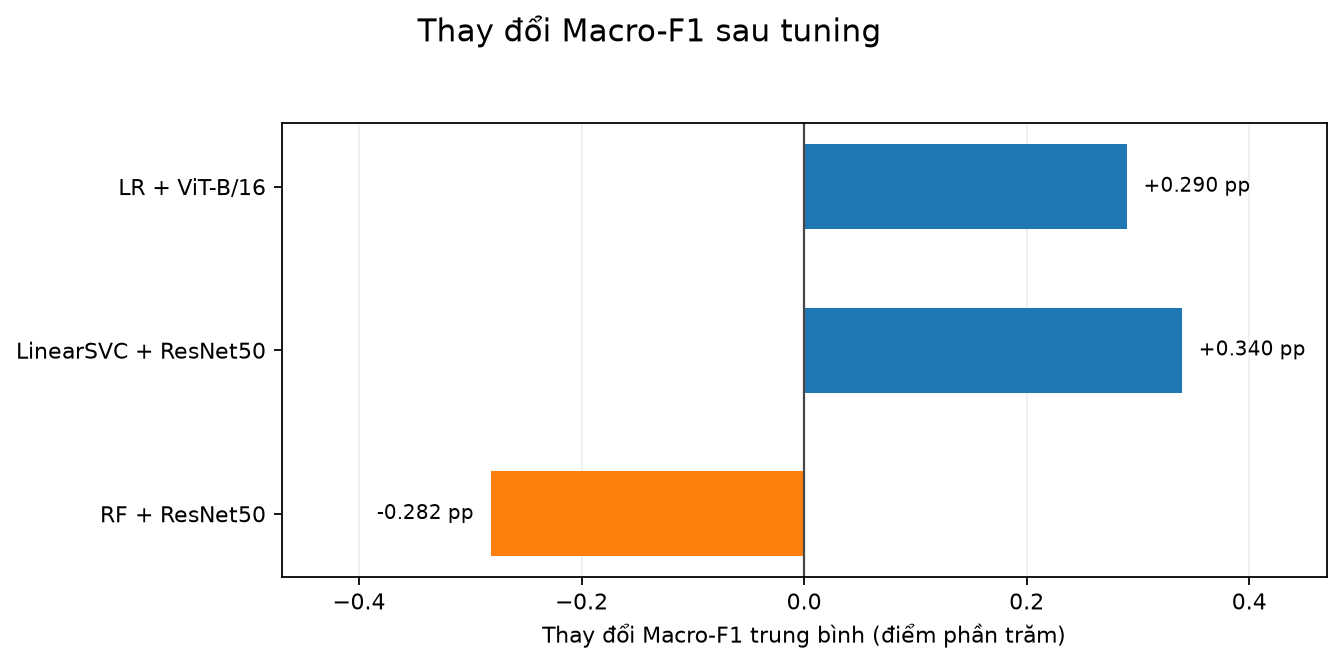
\includegraphics[width=0.89\linewidth]{figures/deep_cell16_out0.png}
    \caption{Mức thay đổi Macro-F1 sau điều chỉnh siêu tham số}
    \label{fig:deep-tune-delta}
\end{figure}

LR chọn $C=0.1$ ở bốn fold và $C=1$ ở fold còn lại. LinearSVC chọn $C=0.003$ ở cả năm fold; đây là giá trị lớn nhất trong lưới đã thử. Sau điều chỉnh, Macro-F1 trung bình của ResNet50 + LinearSVC cao hơn ViT-B/16 + LR khoảng 0.12 điểm phần trăm. LinearSVC đạt Macro-F1 cao hơn LR ở ba fold và thấp hơn ở hai fold, nên chưa đủ căn cứ để khẳng định một cấu hình có hiệu năng cao hơn một cách ổn định trên dữ liệu mới. Với RF, \texttt{min\_samples\_leaf} bằng 1 được chọn ở ba fold và bằng 2 ở hai fold; Macro-F1 trung bình giảm khoảng 0.28 điểm phần trăm. Kết quả cho thấy lựa chọn siêu tham số trên tập xác thực bên trong không bảo đảm cải thiện hiệu năng trên tập xác thực bên ngoài. Các giá trị này đánh giá quy trình lựa chọn siêu tham số trong từng fold, không phải điểm CV của một cấu hình cố định sau bàn giao.

\subsubsection{Phân tích lỗi phân loại dựa trên dự đoán OOF}
\label{subsec:deepoof}
Dự đoán OOF của ViT-B/16 + LR và ResNet50 + LinearSVC sau điều chỉnh siêu tham số được ghép theo MD5 và mã fold. Trong các ma trận nhầm lẫn, hàng là nhãn thật, cột là nhãn dự đoán và màu biểu diễn tỷ lệ theo từng hàng. Các ô không có chú thích tương ứng với số ảnh bằng 0.

\begin{figure}[H]
\centering
\begin{subfigure}[t]{0.45\linewidth}
\centering
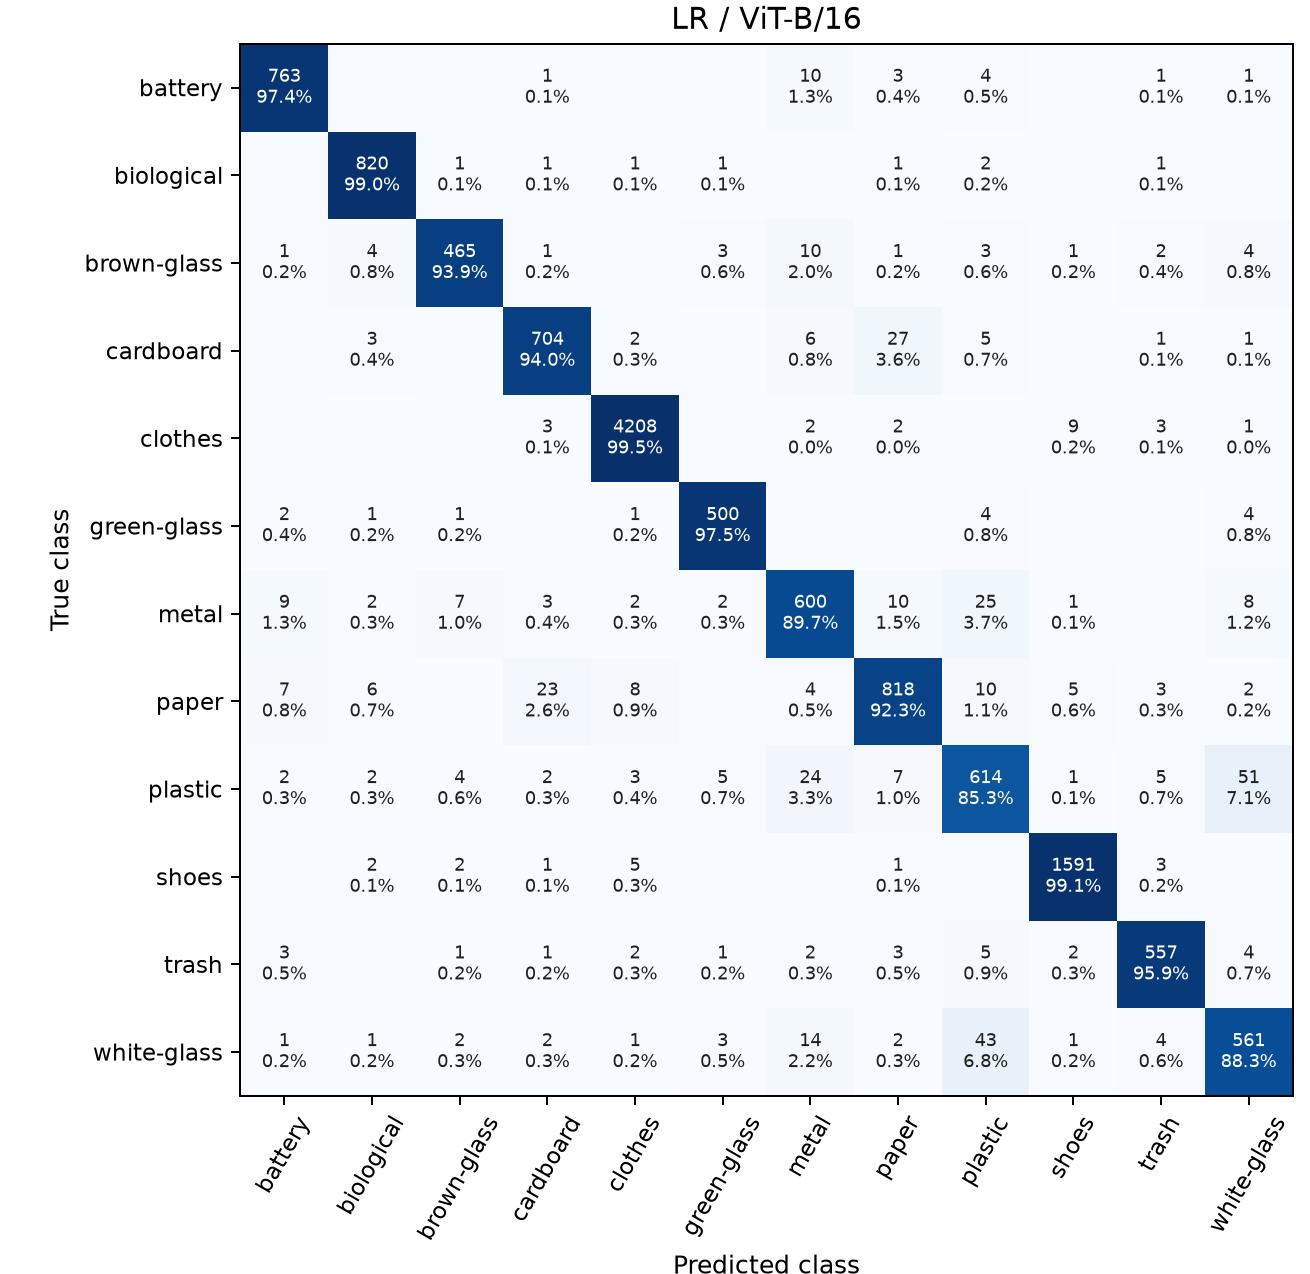
\includegraphics[width=\linewidth]{figures/deep_cell22_out0_panel1.png}
\caption{LR + ViT-B/16.}
\end{subfigure}\hfill
\begin{subfigure}[t]{0.54\linewidth}
\centering
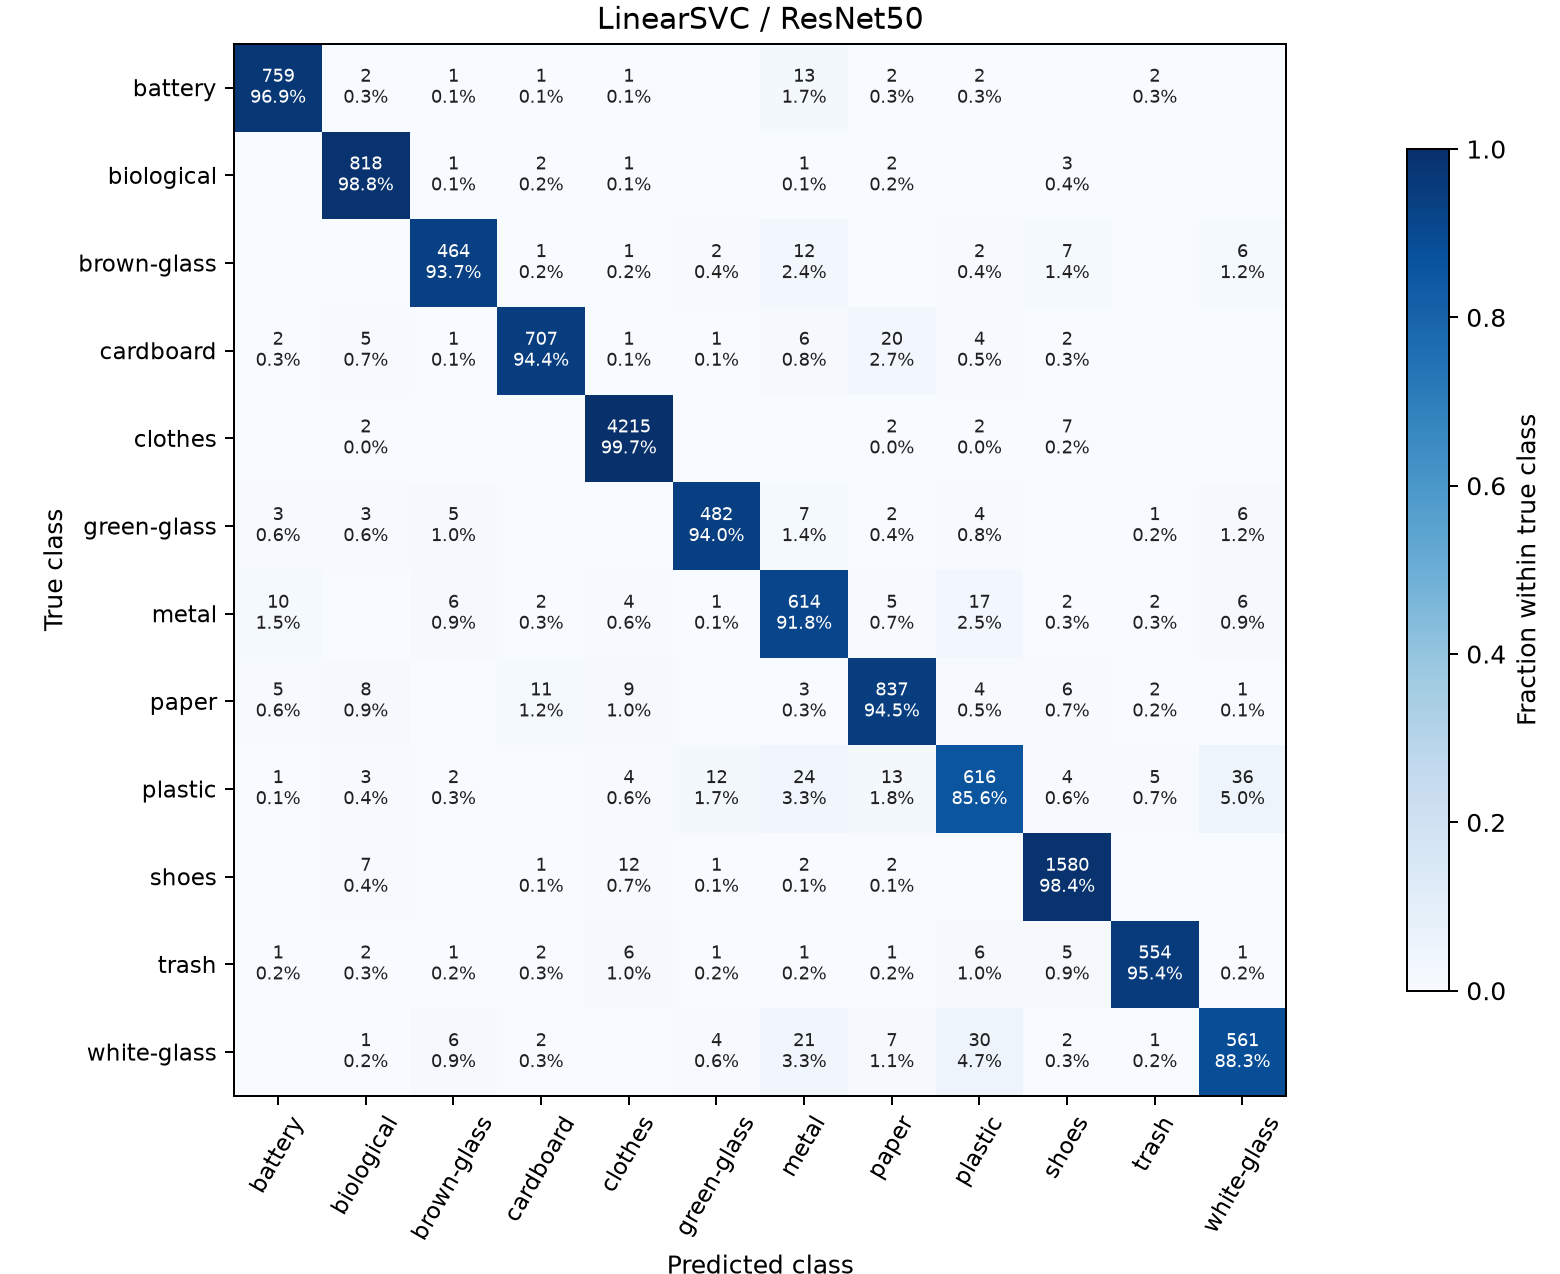
\includegraphics[width=\linewidth]{figures/deep_cell22_out0_panel2.png}
\caption{LinearSVC + ResNet50.}
\end{subfigure}
\caption{Ma trận nhầm lẫn OOF của hai cấu hình sau điều chỉnh siêu tham số.}
\label{fig:deep-cm}
\end{figure}

Hình~\ref{fig:deep-f1-classes} so sánh F1 OOF của sáu lớp có F1 trung bình thấp nhất giữa hai cấu hình. Khi chuyển từ ViT-B/16 + LR sang ResNet50 + LinearSVC, F1 của \texttt{plastic} tăng từ $0.8557$ lên $0.8756$, chủ yếu đi kèm mức tăng Precision (3.79 điểm phần trăm), trong khi Recall chỉ tăng 0.28 điểm phần trăm. Với \texttt{white-glass}, F1 tăng từ $0.8821$ lên $0.8962$; Recall không đổi, nhưng số ảnh thuộc lớp khác bị dự đoán thành \texttt{white-glass} giảm từ 76 xuống 56. Đối với \texttt{metal}, F1 gần như không đổi dù Precision giảm 2.07 và Recall tăng 2.09 điểm phần trăm. Ngoài sáu lớp trong hình, F1 của \texttt{green-glass} giảm 2.49 điểm phần trăm và Recall giảm 3.51 điểm phần trăm. Như vậy, cấu hình đạt Macro-F1 cao hơn không nhất thiết cải thiện kết quả trên mọi lớp; sự khác biệt phản ánh cả đặc trưng lẫn bộ phân loại.

\begin{figure}[H]\centering
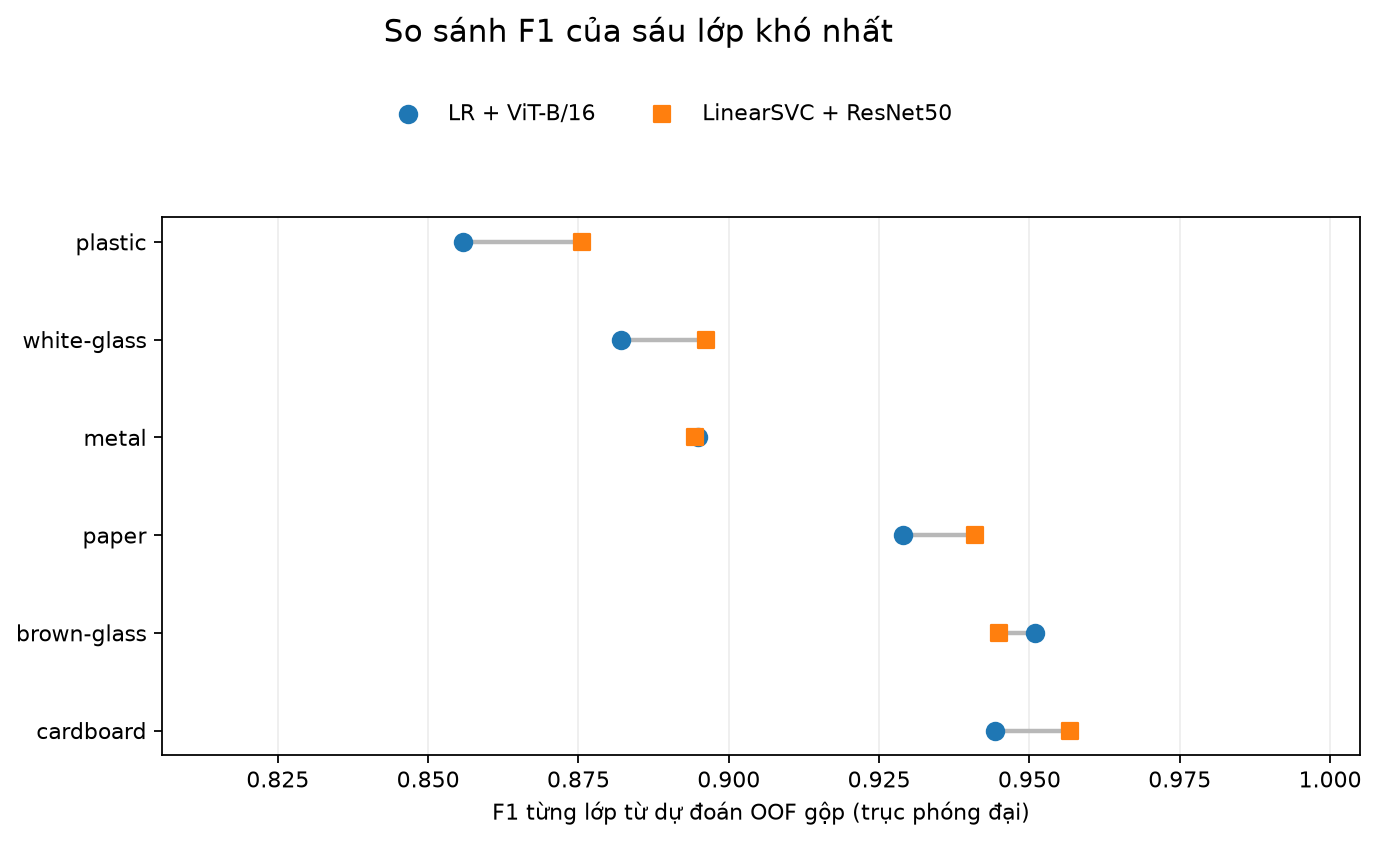
\includegraphics[width=0.8\linewidth]{figures/deep_cell23_out0.png}
\caption{So sánh F1 OOF của sáu lớp có F1 trung bình thấp nhất giữa LR + ViT-B/16 và LinearSVC + ResNet50.}\label{fig:deep-f1-classes}
\end{figure}

\begin{table}[H]\centering\caption{Đối chiếu dự đoán của hai cấu hình học sâu trên cùng 12\,692 ảnh thuộc \textit{development}.}\label{tab:paired}
\small\begin{tabular}{@{}lr@{}}\toprule
Tình huống & Số ảnh\\\midrule
Cả LR và SVC đều đúng & 11\,917\\
LR sai, SVC đúng & 290\\
LR đúng, SVC sai & 284\\
Cả LR và SVC đều sai & 201\\\midrule
\textbf{Tổng} & \textbf{12\,692}\\\bottomrule
\end{tabular}\end{table}

ResNet50 + LinearSVC dự đoán đúng 290 ảnh mà ViT-B/16 + LR dự đoán sai, nhưng dự đoán sai 284 ảnh mà cấu hình LR dự đoán đúng. Tổng số lỗi OOF giảm từ 491 xuống 485 ảnh, tức chỉ giảm 6 ảnh. Với cặp \texttt{plastic} và \texttt{white-glass}, cấu hình LR nhầm 51 ảnh theo hướng plastic$\to$white-glass và 43 ảnh theo hướng ngược lại. Trong 94 lỗi này, cấu hình LinearSVC dự đoán đúng 55 ảnh, tiếp tục nhầm trong cùng cặp ở 31 ảnh và dự đoán sang lớp khác ở 8 ảnh. Đồng thời, LinearSVC phát sinh 35 lỗi mới thuộc cặp này từ những ảnh mà LR không nhầm theo cặp đó. Tổng số lỗi giữa hai lớp vì vậy giảm từ 94 xuống 66; kết quả cho thấy các cấu hình có Macro-F1 gần nhau vẫn mắc lỗi trên những tập ảnh khác nhau.

\subsubsection{Ảnh hưởng của PCA đến hiệu năng phân loại trên ViT-B/16}
\label{subsec:deeppca}
Thí nghiệm giữ cố định ViT-B/16 + LR với $C=1$ và cùng năm fold, chỉ thay đổi bước giảm chiều: không PCA (768 chiều), PCA 512 và PCA 256. Các tham số của \texttt{StandardScaler} và PCA được học từ phần huấn luyện của từng fold. Kết quả được đối chiếu với cấu hình ban đầu $C=1$, không phải quy trình lựa chọn siêu tham số ở Mục~\ref{subsec:deeptune} hoặc cấu hình $C=0.1$ được huấn luyện lại để bàn giao.

% Thoi gian lay tu pca_cv_summary.csv va pca512_cv_summary.csv.
\begin{table}[H]\centering\caption{So sánh PCA trên ViT-B/16 + LR ($C=1$), đánh giá bằng cùng năm fold.}\label{tab:deep-pca}
\small\begin{tabularx}{\linewidth}{@{}Xccc@{}}\toprule
Chỉ số & Gốc 768 & PCA 512 & PCA 256\\\midrule
Macro-F1 (trung bình $\pm$ SD) & $0.9411\pm0.0033$ & $0.9389\pm0.0039$ & $0.9213\pm0.0025$\\
Accuracy & 0.9593 & 0.9582 & 0.9463\\
Phương sai giữ lại & 100\% & 95.83\% & 83.73\%\\
Dung lượng vector (float32) & 3\,072 byte & 2\,048 byte & 1\,024 byte\\
Huấn luyện (s/fold) & 0.52 & 2.01 & 1.42\\
Dự đoán (s/fold) & 0.0097 & 0.0278 & 0.0222\\\bottomrule
\end{tabularx}\end{table}

PCA 512 giảm 33.3\% dung lượng mỗi vector nhưng Macro-F1 giảm khoảng 0.21 điểm phần trăm; PCA 256 giảm 66.7\% dung lượng và làm Macro-F1 giảm khoảng 1.98 điểm phần trăm. Với PCA 256, F1 OOF của \texttt{plastic}, \texttt{white-glass}, \texttt{metal} và \texttt{green-glass} giảm lần lượt 5.02, 4.36, 3.68 và 2.53 điểm phần trăm. Hình~\ref{fig:deep-pca-fold-class} cho thấy Recall cũng giảm không đồng đều: \texttt{white-glass} giảm 3.78 điểm phần trăm, \texttt{metal} giảm 3.74, \texttt{plastic} giảm 3.33, trong khi \texttt{clothes} chỉ giảm 0.17 điểm phần trăm. Do đó, giảm chiều có thể ảnh hưởng đáng kể hơn đến một số lớp so với mức giảm của chỉ số tổng hợp.

\begin{figure}[H]\centering
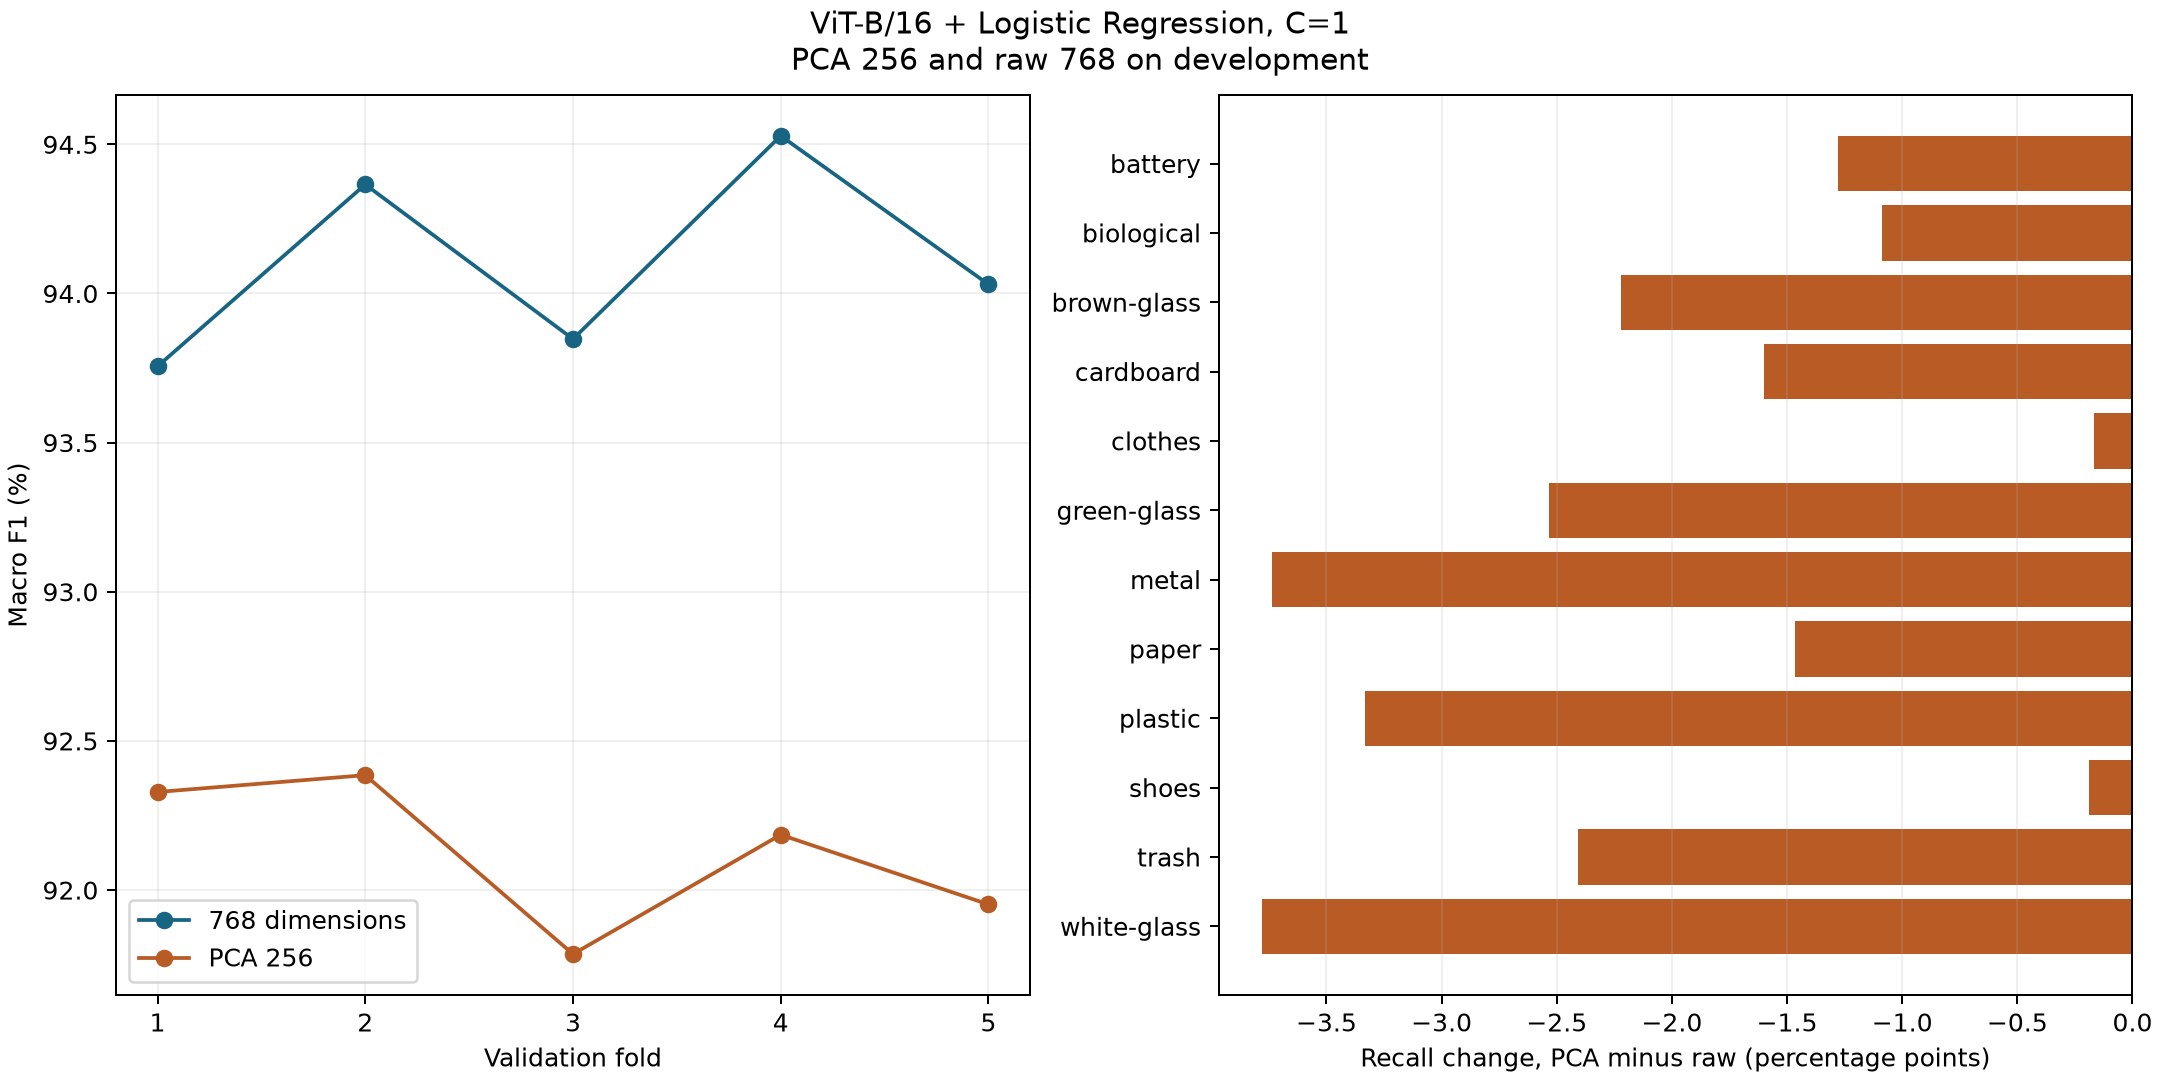
\includegraphics[width=0.97\linewidth]{figures/deep_cell29_out0.png}
\caption{Biến động Macro-F1 theo từng fold và thay đổi Recall theo lớp khi nén từ 768 xuống 256 chiều trên ViT-B/16 + LR}\label{fig:deep-pca-fold-class}
\end{figure}

Tỷ lệ phương sai được giữ lại phản ánh phương sai trong không gian đặc trưng đã chuẩn hóa, không phải tỷ lệ thông tin về nhãn được bảo toàn. Dung lượng mỗi vector trong Bảng~\ref{tab:deep-pca} chưa bao gồm tham số chuẩn hóa và phép chiếu PCA. Riêng ma trận thành phần PCA 512 và PCA 256 lưu dưới dạng float32 lần lượt cần 1\,572\,864 byte và 786\,432 byte. Vì vậy, giảm dung lượng mỗi vector không đồng nghĩa giảm tổng dung lượng pipeline. Thời gian fit trong bảng bao gồm chuẩn hóa, PCA (nếu có) và huấn luyện LR; thời gian dự đoán gồm các bước biến đổi tương ứng và dự đoán nhãn. PCA 512 được chạy bổ sung ở lượt thực nghiệm riêng nên không diễn giải các chênh lệch thời gian nhỏ như kết quả benchmark được kiểm soát. Trong các phép đo đã lưu, cả hai cấu hình PCA đều có thời gian fit cao hơn cấu hình không PCA.

\subsubsection{Các cấu hình được chọn cho bước đánh giá cuối cùng}
Hai cấu hình được chọn để đánh giá cuối cùng gồm ViT-B/16 + LR ($C=0.1$) và ResNet50 + LinearSVC ($C=0.003$). Cả hai có Macro-F1 gần nhau nhưng khác nhau về lỗi theo lớp; ViT-B/16 + LR có số chiều đặc trưng thấp hơn và thời gian huấn luyện bộ phân loại thấp hơn trong các phép đo đã thực hiện. Với LR, $C=0.1$ được chọn bằng phép chia xác thực trên dev trước khi huấn luyện lại; với LinearSVC, $C=0.003$ được chọn nhất quán trong năm fold ngoài. Hai pipeline được huấn luyện lại trên toàn bộ 12\,692 ảnh dev. Điểm CV ở Mục~\ref{subsec:deeptune} không phải kết quả đánh giá độc lập của các pipeline đã huấn luyện lại; final test thuộc bước đánh giá chung của nhóm.

\subsection{Đối chiếu kết quả hai hướng phân loại}
\label{sec:compare}
\subsubsection{So sánh kết quả phân loại tổng thể}
Bảng~\ref{tab:cross} tổng hợp các cấu hình đại diện của hai hướng, gồm kết quả ban đầu, sau điều chỉnh siêu tham số và sau giảm chiều PCA. Mọi giá trị đều được đánh giá trên \textit{development}, không phải tập kiểm tra cuối cùng. Cùng dùng Macro-F1 không đồng nghĩa hai hướng áp dụng cùng quy trình lựa chọn mô hình; điểm khác biệt được phân tích ở Mục~\ref{sec:threats}.

\begin{table}[H]\centering\caption{So sánh các cấu hình đại diện trên tập dev. Macro-F1 được trình bày dưới dạng trung bình $\pm$ SD; các chỉ số còn lại là trung bình qua năm fold.}\label{tab:cross}
\small\setlength{\tabcolsep}{3.5pt}
\begin{tabularx}{\linewidth}{@{}Xcccc@{}}\toprule
Cấu hình & Macro-F1 & Accuracy & Macro-P & Macro-R\\\midrule
Dummy most-frequent & $0.0416\pm0.0000$ & 0.3331 & 0.0278 & 0.0833\\\midrule
SIFT-BoVW + LR & $0.5110\pm0.0109$ & 0.6079 & 0.5065 & 0.5241\\
SIFT-BoVW + SVM RBF & $0.5718\pm0.0041$ & 0.6791 & 0.5920 & 0.5599\\
SIFT-BoVW + PCA 256 + SVM RBF & \textbf{$0.5744\pm0.0055$} & 0.6812 & 0.5906 & 0.5657\\
HOG + PCA 128 + SVM RBF & $0.5499\pm0.0096$ & 0.6748 & 0.5654 & 0.5444\\\midrule
ViT-B/16 + LR (sau tuning) & $0.9440\pm0.0037$ & 0.9613 & 0.9450 & 0.9434\\
ResNet50 + LinearSVC (sau tuning) & \textbf{$0.9451\pm0.0030$} & 0.9618 & 0.9482 & 0.9429\\
ResNet50 + RF (sau tuning) & $0.9061\pm0.0050$ & 0.9332 & 0.9157 & 0.8985\\\bottomrule
\end{tabularx}
\par\smallskip\footnotesize Macro-P và Macro-R lần lượt là Macro-Precision và Macro-Recall. SD của các cấu hình truyền thống dùng \texttt{ddof=0}; SD của các cấu hình học sâu và Dummy trong bảng này dùng \texttt{ddof=1}. Kết quả sau tuning là kết quả quy trình lựa chọn siêu tham số theo từng fold ngoài.
\end{table}

\begin{figure}[H]\centering
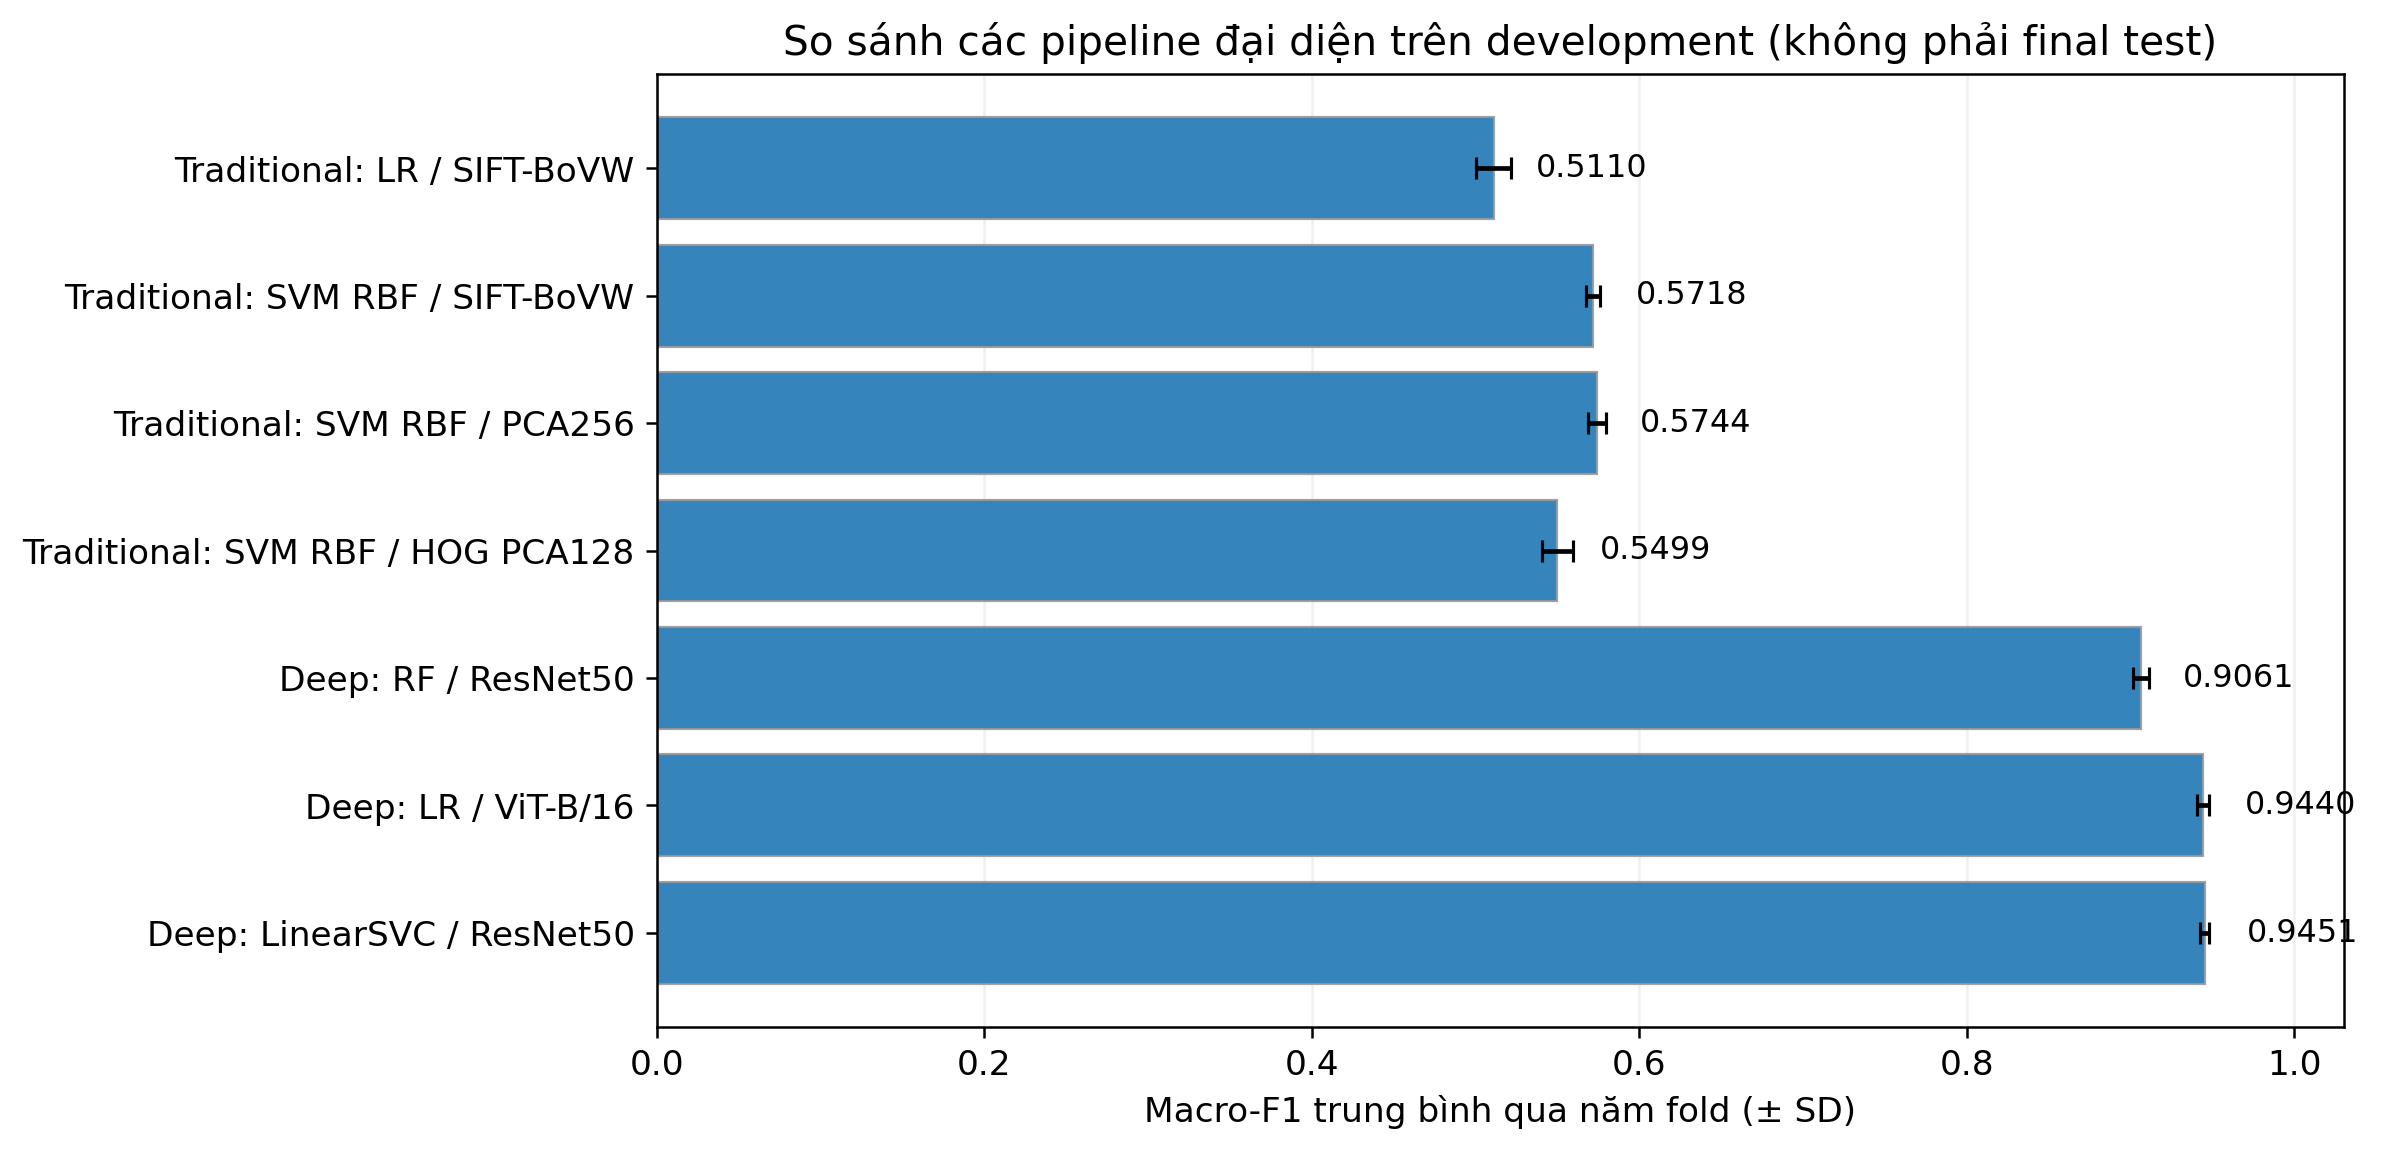
\includegraphics[width=0.96\linewidth]{figures/comparison_selected.png}
\caption{So sánh Macro-F1 của các cấu hình đại diện trên \textit{development}}\label{fig:comparison-selected}
\end{figure}

Trong phạm vi các cấu hình đã khảo sát, SIFT-BoVW + PCA 256 + SVM RBF đạt Macro-F1 trung bình cao nhất ở hướng truyền thống ($0.5744$), còn ResNet50 + LinearSVC sau điều chỉnh siêu tham số dẫn đầu hướng học sâu ($0.9451$). Chênh lệch Macro-F1 trung bình là khoảng 37.07 điểm phần trăm trên dev. Đây là chênh lệch giữa hai cấu hình hoàn chỉnh, không phải ước lượng riêng ảnh hưởng của phương pháp trích xuất đặc trưng.

\subsubsection{Phân tích vai trò của biểu diễn và bộ phân loại}
Đối chiếu theo từng họ bộ phân loại cho thấy ngay cả các cấu hình học sâu ban đầu cũng đạt Macro-F1 cao hơn các cấu hình truyền thống sau điều chỉnh siêu tham số trong phạm vi khảo sát (Bảng~\ref{tab:trad-six} và Bảng~\ref{tab:deep9}). Với LR, giá trị cao nhất trên đặc trưng học sâu là $0.9411$ so với $0.5110$ trên đặc trưng truyền thống; với SVM là $0.9417$ so với $0.5718$; với RF là $0.9089$ so với $0.4899$. Tuy nhiên, các họ bộ phân loại này khác về siêu tham số, trọng số lớp và biến thể SVM, nên đây là đối chiếu mô tả, không phải thí nghiệm chỉ thay đổi đặc trưng.

Các bộ phân loại tuyến tính đạt kết quả cao trên cả ba đặc trưng học sâu, trong khi RF thấp hơn. Một cách giải thích có thể là các mô hình tiền huấn luyện đã tạo ra biểu diễn giúp phân biệt các lớp bằng ranh giới quyết định tuyến tính. Tuy nhiên, thí nghiệm chưa đo trực tiếp khả năng phân tách giữa các lớp trong không gian đặc trưng, nên đây chỉ là giả thuyết giải thích kết quả.

\subsubsection{So sánh lỗi phân loại và vai trò của thông tin màu}
Ở hướng truyền thống, SIFT-BoVW + SVM RBF thường nhầm \texttt{green-glass} với \texttt{brown-glass} theo cả hai hướng; F1 của \texttt{green-glass} chỉ khoảng $0.357$. Thí nghiệm HOG kết hợp histogram màu HSV cho thấy cải thiện Macro-F1 10.87 điểm phần trăm, nhưng chưa xác định mức cải thiện riêng trên từng lớp thủy tinh. Ở hai cấu hình học sâu được chọn, nhầm lẫn giữa \texttt{plastic} và \texttt{white-glass} vẫn nổi bật dù Macro-F1 tổng thể cao. Chưa có thí nghiệm loại bỏ thông tin màu trên đặc trưng học sâu để đối chiếu riêng ảnh hưởng của màu sắc.

Phép đối chiếu trên dựa vào các ma trận nhầm lẫn và chỉ số tổng hợp của từng hướng. Dự đoán OOF giữa hai hướng chưa được ghép theo MD5 để kiểm tra từng ảnh, nên chưa xác định được những ảnh cụ thể được dự đoán đúng thêm khi chuyển sang đặc trưng học sâu.

\subsubsection{Đối chiếu hiệu quả giảm chiều và chi phí tính toán}
Hiệu quả giảm chiều phụ thuộc vào loại đặc trưng và bộ phân loại. Trên SIFT-BoVW + SVM RBF, giảm từ 500 xuống 128 chiều giúp duy trì Macro-F1 gần với cấu hình không PCA; trên ViT-B/16 + LR, giảm từ 768 xuống 512 chiều làm Macro-F1 giảm khoảng 0.21 điểm phần trăm, còn giảm xuống 256 chiều làm chỉ số này giảm khoảng 1.98 điểm phần trăm. Không có một số chiều PCA phù hợp cho mọi cấu hình. Việc giữ lại tỷ lệ phương sai cao cũng không bảo đảm duy trì đầy đủ thông tin hữu ích cho phân loại.

Về chi phí tính toán, hướng truyền thống cần trích xuất HOG hoặc SIFT từ ảnh; hướng học sâu cần chạy mô hình tiền huấn luyện để tạo vector đặc trưng trước khi phân loại. Thời gian huấn luyện các bộ phân loại được đo trong những điều kiện phần cứng và mức chạy song song chưa đồng nhất, đồng thời thường không bao gồm thời gian trích xuất đặc trưng. Do đó, không thể kết luận toàn bộ quy trình học sâu nhanh hơn hay chậm hơn hướng truyền thống chỉ dựa trên thời gian huấn luyện bộ phân loại. Để đánh giá chi phí triển khai, cần đo thời gian xử lý từ ảnh đầu vào đến dự đoán, mức sử dụng RAM lớn nhất, dung lượng mô hình và số ảnh xử lý mỗi giây trên cùng phần cứng.

\subsection{Thảo luận về độ tin cậy và giới hạn đánh giá}
\label{sec:threats}
\subsubsection{Rò rỉ dữ liệu và tính độc lập của đánh giá}
Ở cả hai hướng, các tham số chuẩn hóa và PCA (nếu có) được ước lượng từ phần huấn luyện của từng fold. Tuy nhiên, từ điển SIFT-BoVW được học bằng \texttt{MiniBatchKMeans} trên tập train ban đầu rồi dùng để mã hóa toàn bộ dữ liệu, trước khi thực hiện CV trên dev (train và validation). Do đó, một số ảnh xác thực trong từng fold đã tham gia vào tập dữ liệu dùng để học từ điển. Dù quá trình học từ điển không sử dụng nhãn, thông tin từ ảnh xác thực vẫn có thể ảnh hưởng đến biểu diễn đặc trưng. Đây là rò rỉ dữ liệu ở bước học từ điển trong quy trình CV; việc đặt \texttt{StandardScaler} và PCA trong pipeline không khắc phục được vấn đề này.

Mức ảnh hưởng đến Macro-F1 chưa được định lượng. Để đánh giá chặt chẽ hơn, cần học lại từ điển BoVW chỉ từ ảnh thuộc phần huấn luyện của mỗi fold rồi mã hóa phần xác thực bằng từ điển đó. Các kết quả hiện tại vì vậy chỉ được sử dụng để khảo sát trên dev. Từ điển không được học từ final test; tập kiểm tra cuối cùng cần được sử dụng sau khi các cấu hình đã được chốt.

\subsubsection{Thiên lệch lựa chọn mô hình và khác biệt trong quy trình đánh giá}
Hướng truyền thống thử nhiều $C$, $\alpha$, độ sâu cây, loại hàm nhân và số chiều PCA rồi dùng chính năm fold để chọn mô hình có điểm trung bình cao nhất. Cách lựa chọn này có thể gây thiên lệch do chọn mô hình (selection bias): kết quả của cấu hình được chọn trên chính các fold đó không phải ước lượng độc lập cho toàn bộ quy trình lựa chọn. Hướng học sâu dùng tập xác thực bên trong từng fold ngoài để chọn siêu tham số, nhưng ba cặp đặc trưng - bộ phân loại được khảo sát tiếp cũng được chọn dựa trên kết quả CV ở cùng \textit{development}. Vì vậy cả hai hướng đều phải hạn chế kết luận ở mức khảo sát trên \textit{development}.

Hai hướng còn khác nhau về trọng số lớp, kích thước ảnh đầu vào, kiến trúc trích xuất và biến thể bộ phân loại. LR và SVM truyền thống dùng trọng số lớp cân bằng, RF truyền thống dùng \texttt{balanced\_subsample}, còn các bộ phân loại học sâu không dùng trọng số lớp. Do đó, chênh lệch quan sát được phản ánh hiệu năng của các cấu hình đã khảo sát, chưa xác định riêng ảnh hưởng của phương pháp trích xuất đặc trưng.

\subsection{Kết luận}
\label{sec:concl}
Trên tập dev, các cấu hình sử dụng đặc trưng học sâu đạt Macro-F1 cao hơn các cấu hình sử dụng đặc trưng truyền thống trong phạm vi khảo sát. ResNet50 + LinearSVC sau điều chỉnh siêu tham số đạt Macro-F1 trung bình cao nhất ($0.9451$), so với $0.5744$ của SIFT-BoVW + PCA 256 + SVM RBF ở hướng truyền thống.

Hiệu năng phụ thuộc vào sự kết hợp giữa đặc trưng và bộ phân loại. SVM RBF đạt kết quả cao nhất trên SIFT-BoVW, trong khi LR và LinearSVC đạt kết quả cao trên cả ba đặc trưng học sâu. Điều chỉnh siêu tham số cải thiện kết quả của hai cấu hình tuyến tính được khảo sát tiếp ở hướng học sâu, nhưng không cải thiện kết quả RF trên ResNet50. Bổ sung histogram màu vào HOG cũng cho mức cải thiện đáng kể trong cấu hình LR đã thử.

Phân tích dự đoán OOF cho thấy nhầm lẫn giữa các lớp thủy tinh và nhựa vẫn cần được chú ý. Hai cấu hình học sâu có Macro-F1 cao nhất mắc lỗi trên những tập ảnh không hoàn toàn giống nhau; cấu hình có Macro-F1 cao hơn không cải thiện đồng thời mọi lớp.

Đối với giảm chiều, SIFT-BoVW + SVM RBF duy trì Macro-F1 gần với cấu hình không PCA khi giảm từ 500 xuống 128 chiều. ViT-B/16 + LR với PCA 512 giảm 33.3\% dung lượng mỗi vector và giảm khoảng 0.21 điểm phần trăm Macro-F1, nhưng không làm giảm thời gian fit trong các phép đo hiện có. Hiệu quả của PCA vì vậy cần được xem xét đồng thời theo hiệu năng phân loại và chi phí tính toán.
